% \documentclass[print]{gescons} % Quando for enviar para a gráfica
\documentclass[a4paper]{gescons}

\magazinename  {GENSCONS}
\magazinetheme {Special GitHub issue}
\magazinevolume{7}
\magazineissue {20XX}

\begin{document}
    % \frontpage{images/capa}{15}{15}
    %\% frontpage{images/capa.pdf}{15}{15}
    %\frontpage{images/capa.pdf}{0}{0}

    \tableofcontents

    \documentclass{gescons}

\genre {Editorial}
\author{Amanda Vieira}
\title{20 anos de Publicação Interassistencial: Passado, Presente e Futuro da Editares}

\begin{document}
    \makeentrevistatitle
    %\maketitle

    %\fullwidthimage{fields}{b}

    \coverart{back/editorial}
    %\coverart{../fundo-generico.png}

    \begin{multicols}{2}

%\begin{center}
%    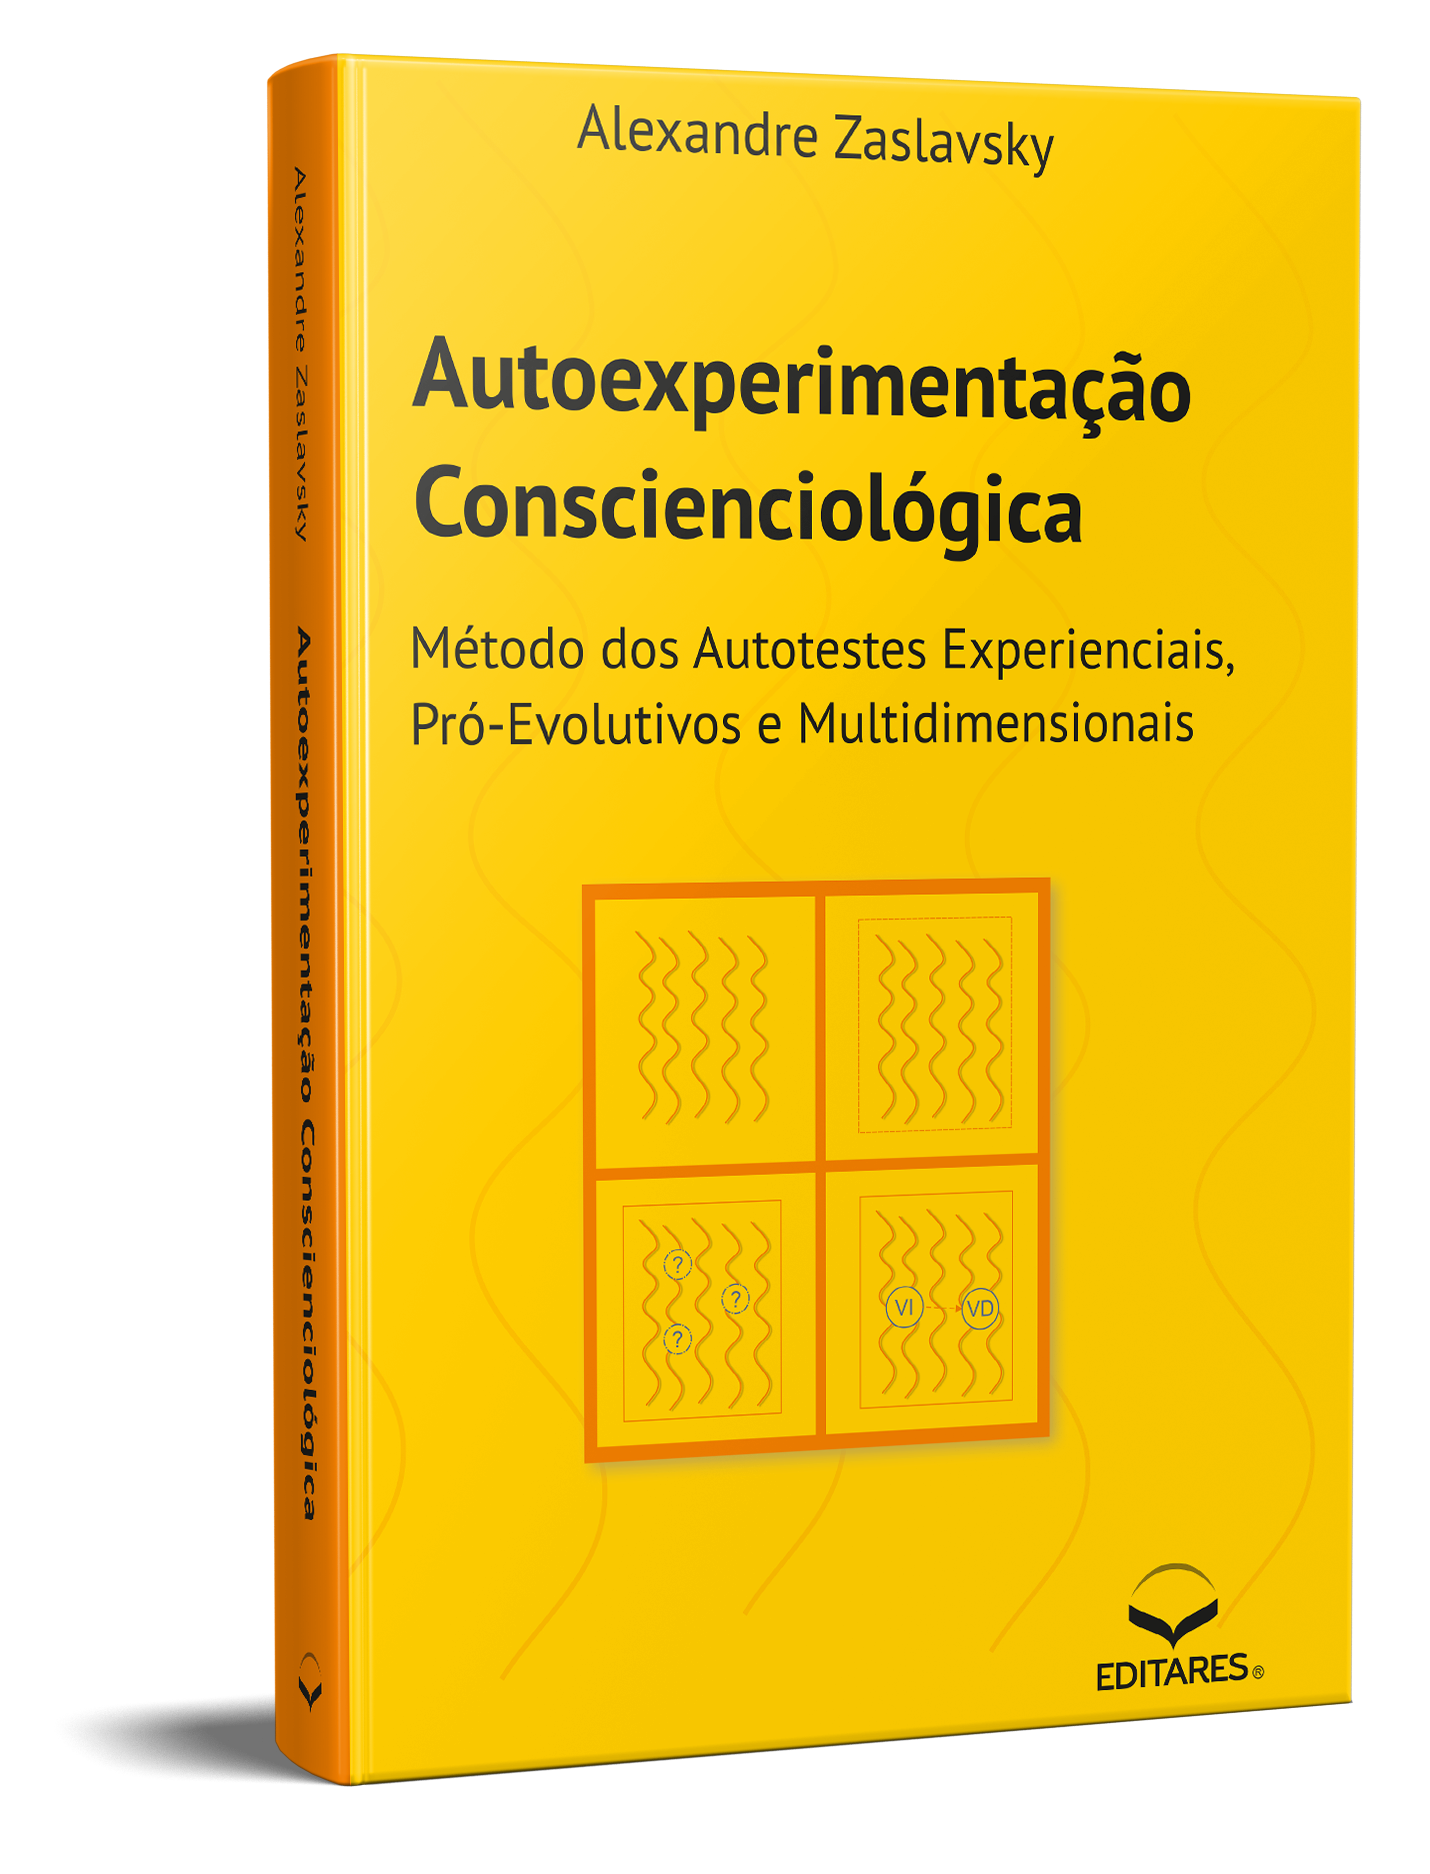
\includegraphics[width=4cm]{articles/entrevista/mockups/Alexandre-Zas.png}
%\end{center}

Em 2024, a Editares completou 20 anos de dedicação à publicação técnico-científica de obras conscienciológicas. Duas décadas de trabalho tarístico, construídas por muitas mãos, em que cada autor, revisor, diagramador, conselheiro, voluntário e leitor fez parte de um mesmo propósito: \textbf{expandir o esclarecimento e favorecer a evolução das consciências por meio da escrita.}

Celebrar essa história significa reconhecer o valor do esforço coletivo. Desde os primeiros livros publicados até os mais recentes lançamentos, cada obra representa um marco de interassistência, registrando aprendizados, reflexões e contribuições para o desenvolvimento da Conscienciologia e para a maxiproéxis grupal.

Esta edição da Revista Gescons propõe um olhar integrado sobre a trajetória da Editares: passado, presente e futuro se encontram para inspirar novos desafios e conquistas. É um convite para pensar no que já realizamos juntos e, principalmente, no que ainda podemos alcançar coletivamente.

Na primeira seção, apresentamos \textbf{resumo do biênio} com os acontecimentos mais relevantes da Editares entre 2023 e 2024: a conquista da Certificação Institucional da UNICIN, a participação no Congraçamento das ICs, a distribuição internacional de materiais no Japão e na Europa, as atualizações do fluxo editorial e os números que refletem nossa produção recente. Um destaque especial vai para a listagem completa dos voluntários atuais, organizados por equipes de trabalho, valorizando quem faz a Editares acontecer.

Na segunda seção, trazemos \textbf{atualizações} e novidades institucionais: a criação da Escola de Editores, voltada à formação e qualificação de novos voluntários; as novas estratégias de marketing; a nova revista científica da Editares para expansão da especialidade Editoriologia e Publicaciologia; a reativação da parceria com o IIPC para ampliar a venda de livros; e os grupos de trabalho com a UNICIN, responsáveis por repensar processos comerciais e editoriais.

Por fim, na terceira seção, apresentamos os \textbf{lançamentos de 2024 e 2025,} com obras que ampliam o debate técnico e aprofundam a pesquisa conscienciológica.

Mais do que celebrar o passado, esta edição propõe \textbf{um olhar para o futuro.} Queremos inspirar novos autores, atrair mais voluntários e consolidar práticas editoriais cada vez mais qualificadas e interassistenciais. Seguimos firmes no propósito de transformar ideias em livros, livros em esclarecimento e esclarecimento em evolução.

Agradecemos a todos os voluntários, autores, leitores e parceiros que fazem parte desta história. Que os próximos anos sejam ainda mais produtivos, lúcidos e interassistenciais.

Boa leitura!



%\begin{center}
%    %  trim={<left> <lower> <right> <upper>}
%    
\includegraphics[width=8cm,trim={0 200 0 70},clip]{articles/inicial/imagens/Amanda.jpeg}
%\end{center}

%\begin{pullquote}
%``A escrita de uma obra conscienciológica é uma oportunidade evolutiva inigualável.''
%\end{pullquote}

        
    \end{multicols}

\begin{figure}[h] % [htbp] are placement options (here, top, bottom, page)
\centering % Centers the image and caption

\includegraphics[width=5cm,trim={0 200 0 70},clip]{articles/inicial/imagens/Amanda.jpeg}
\caption*{Editora desta Edição} % The caption text
\end{figure}

\end{document}

    \documentclass{gescons}

\genre {Resumo do Biênio}
\author{Ana Claudia Prado e Magda Stapf Amancio}
\title{Gestão 2024-2025: Entrevista com as Coordenadoras}

\begin{document}
    \makeentrevistatitle
    %\maketitle

    %\fullwidthimage{fields}{b}

    %\coverart{back/editorial}
    \coverart{../fundo-generico.png}

    \begin{multicols}{2}

%\begin{center}
%    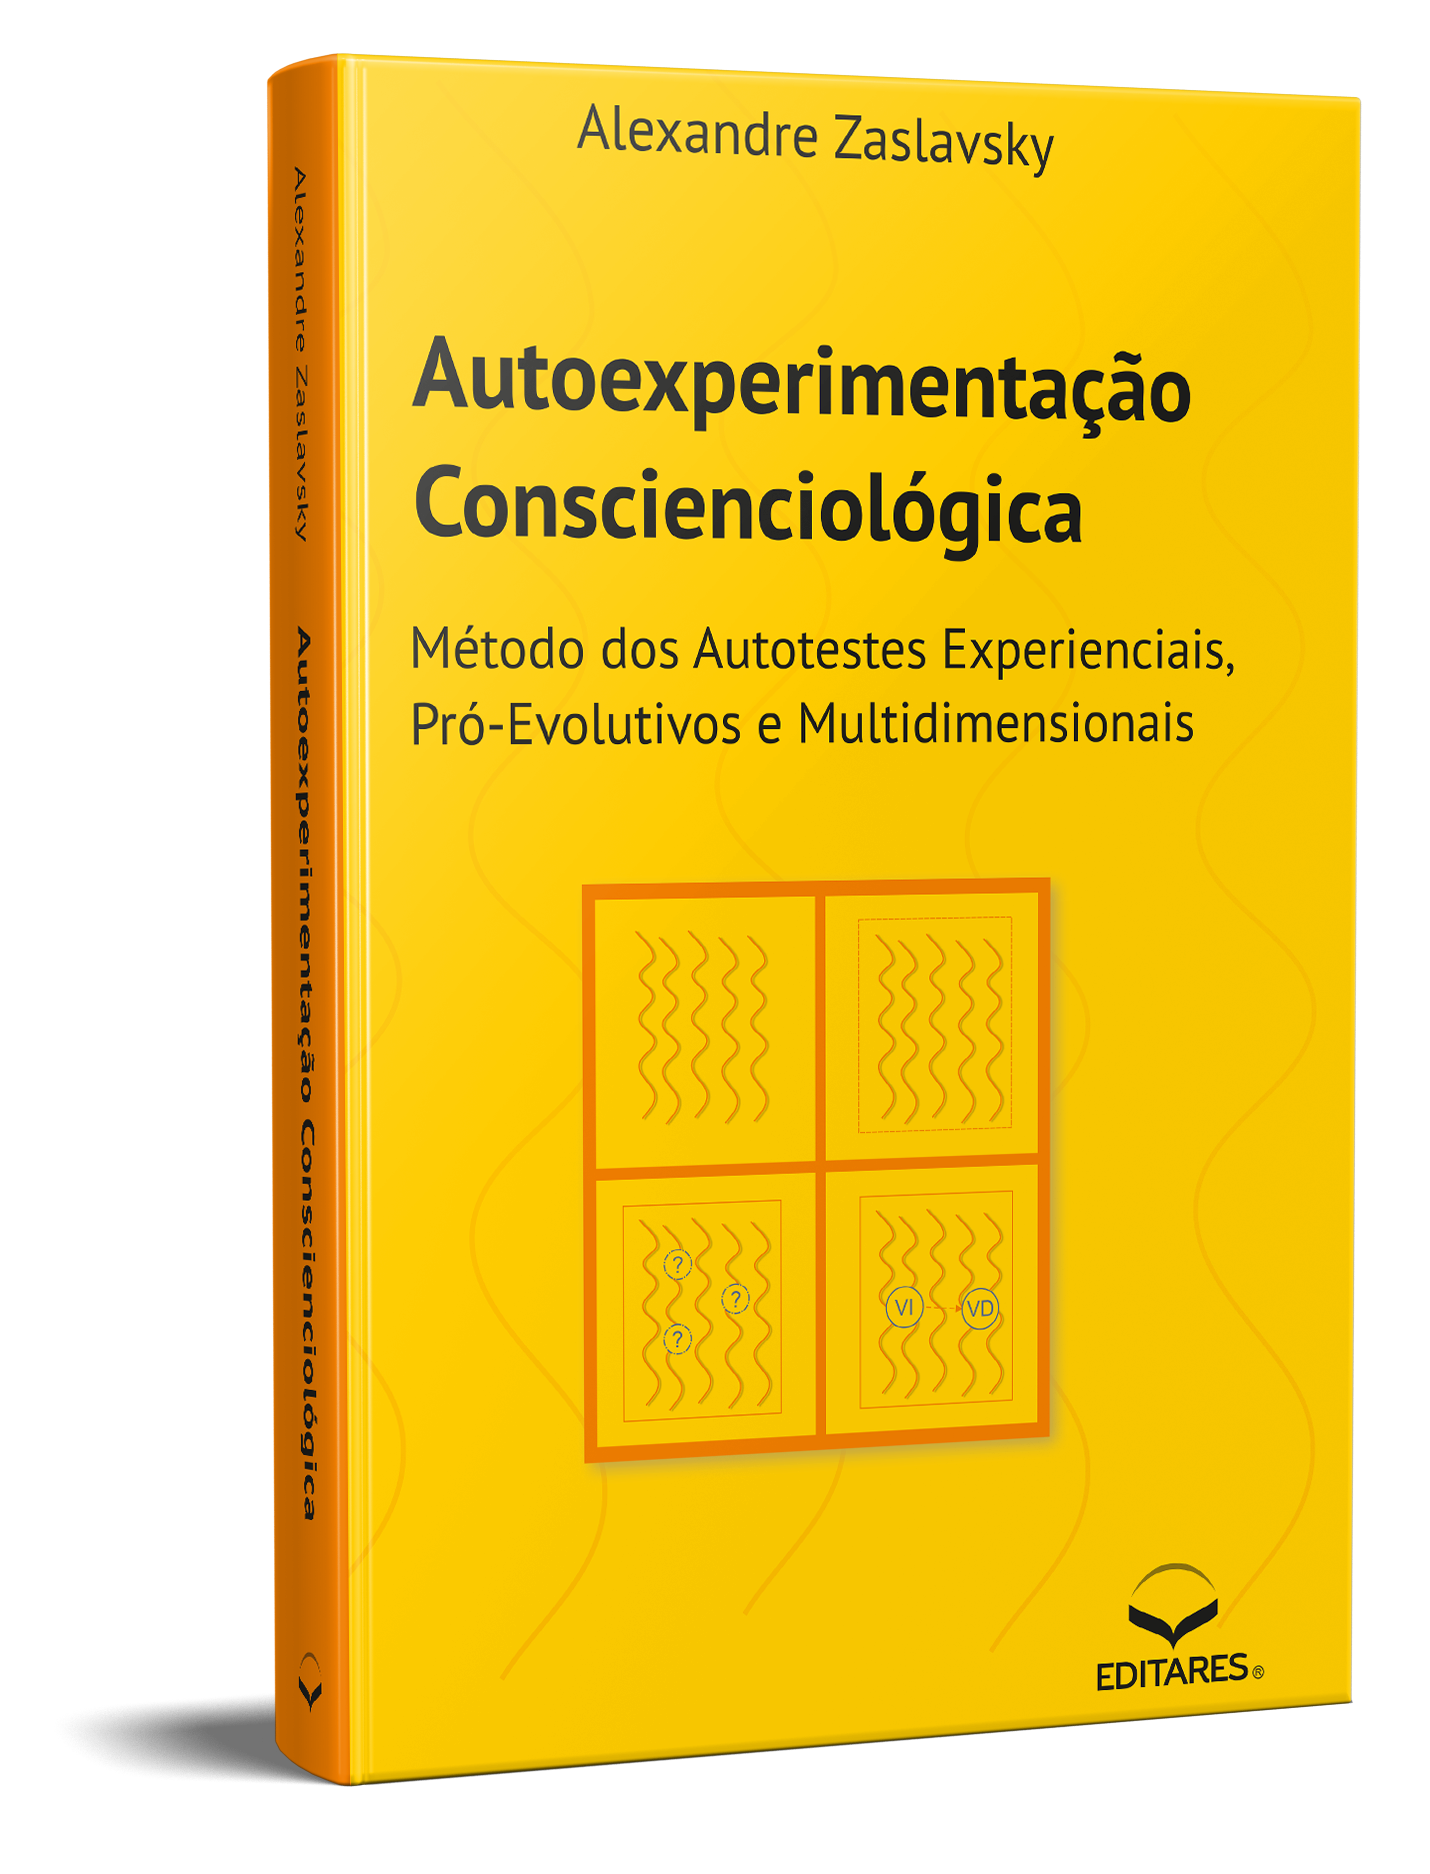
\includegraphics[width=4cm]{articles/entrevista/mockups/Alexandre-Zas.png}
%\end{center}

    \begin{center}
        %  trim={<left> <lower> <right> <upper>}
        
\includegraphics[width=8cm,trim={100 0 100 1100},clip]{articles/resumo/fotos/materia2/IMG20241208144410.jpg}
    \end{center}



\textbf{Como foi o convite ou o processo de chegada de vocês à coordenação da Editares? Quais eram suas expectativas ao assumir e como elas se confirmaram ou mudaram nesses dois anos?}

\textbf{Ana:} Foi um convite bastante refletido. Precisei pensar muito antes de aceitar, porque já tinha diversas atividades. Houve um grande investimento da liderança da Editares para que eu assumisse a coordenação, e uma condição era ter coordenação em dupla. Então, Cristina Ellwanger convidou a Magda.

\textbf{Magda:} Eu já tinha decidido que só toparia se fosse com a Ana. Se ela aceitasse, eu ficaria junto.

\textbf{Ana:} No início, eu não tinha muitas expectativas. As ideias foram surgindo com o tempo e fomos fazendo acontecer. Começamos organizando os contratos de cessão de direitos e planejando a mudança da sala, para acomodar melhor a equipe e atender os autores e neo-autores.

\textbf{Magda:} Eu tinha feito o curso de preparação de lideranças da Unicin, mas na época não compreendia bem o que representava. No curso, cheguei a dizer que não assumiria nenhuma gestão. Perguntaram do que eu estava me escondendo --- e essa pergunta ficou ecoando, me fazendo refletir.

\textbf{Ana:} Eu também não pensava em coordenação, nem em voluntariar na Editares. Mas, ao publicar o livro Antologia da Técnica de Mais 1 Ano de Vida Intrafísica, juntamente com mais 3 organizadoras, senti vontade de ajudar mais, pois me identifiquei com o trabalho. Aos poucos, percebi o quanto isso se conectava com a minha proéxis: auxiliar outras pessoas a escreverem seus livros.

\begin{pullquote}
``Aos poucos, percebi o quanto isso se conecta com a minha proéxis: auxiliar outras pessoas a escreverem seus livros.''
\end{pullquote}

\textbf{Quais foram os maiores desafios enfrentados na gestão da editora nesse período? Que aprendizados pessoais e grupais vocês destacariam dessa experiência?}

\textbf{Ana:} Um dos maiores desafios foi formar equipes e reestruturar o Conselho Editorial e o fluxo editorial. Outro, foi dar mais celeridade às publicações preservando a qualidade. Isso só foi possível graças ao envolvimento dos voluntários, autores, editores e de voluntários da CCCI. Mostramos do que somos capazes quando trabalhamos juntos. Conseguimos organizar o fluxo de chegada das obras, fazer o acompanhamento até a publicação e manter um bom ritmo. Essa “máquina” só funciona porque contamos com especialistas para revisão, conferência e apoio editorial. Hoje, tudo flui bem em razão do esforço coletivo.

\textbf{Magda:} Essa experiência exigiu um amadurecimento na gestão, porque tivemos que desenvolver uma visão de conjunto. Para mim, um desafio marcante foi a perda das informações  do sistema de gestão de vendas dos livros. Perdemos dados atualizados e tivemos que fazer um esforço enorme para recuperá-los. Trabalhei lado a lado com a Angélica {[funcionária da Editares]} nessa fase. A Ana estava viajando, e isso acabou ajudando, porque ela conseguia me acalmar e me manter focada na solução. Essa parceria na coordenação funcionou muito bem: quando uma estava sobrecarregada, a outra dava suporte.

\textbf{Que efeitos essa experiência trouxe para a autopesquisa e a proéxis de cada uma?}

\textbf{Ana:} Para mim, foi como se eu tivesse me localizado na proéxis. É como se tivesse feito um ``download'' não só da intermissão, mas também de experiências de outras vidas. Estar na linha de frente, na ``vitrine'', não era algo natural para mim. Aprendi a lidar com a exposição, a assumir responsabilidades com mais maturidade e a mostrar quem eu realmente sou --- com meus traf\emph{o}res, traf\emph{a}res e traf\emph{ai}s. Um dos maiores aprendizados foi não limitar meus potenciais por medo de errar ou aparecer. A vivência me ajudou a superar essas barreiras internas.

\textbf{Magda:} Para mim, a gestão ampliou muito minha visão. Passei a enxergar melhor o funcionamento do grupo, amadureci e desenvolvi um senso maior de pertencimento à Comunidade Conscienciológica. Essa sensação de estar integrada e contribuir para algo maior é muito gratificante.

\textbf{Como vocês imaginam o futuro da editoração conscienciológica?}

\textbf{Ana:} Gostaria que conseguíssemos dar ainda mais celeridade às publicações. Para isso, precisamos que as obras cheguem mais bem estruturadas, o que permitiria avançar com mais rapidez sem perder a qualidade. Estamos trabalhando nesse sentido.

\textbf{Magda:} A parceria com a Uniescon pode contribuir bastante nesse processo.

\textbf{Ana:} Além disso, seria importante ampliar o engajamento de voluntários da CCCI, especialmente aqueles com disponibilidade para atuar nas revisões.

\textbf{Que mensagem final gostariam de deixar para os leitores e voluntários da Conscienciologia?}

\textbf{Ana:} Se uma oportunidade ou desafio bater à sua porta, abrace-o e leve até o fim. No final, reflita: \emph{o que aprendi com isso?}

\begin{pullquote}
``Se uma oportunidade ou desafio bater à sua porta, abrace-o e leve até o fim. No final, reflita: \emph{o que aprendi com isso?}''
\end{pullquote}

\textbf{Magda:} Apesar dos desafios da coordenação, esse trabalho vale muito a pena. Ele contribui diretamente para o amadurecimento pessoal, grupal e intraconsciencial.

\coverart{../fundo-generico.png}

\textbf{Coordenadoras:} Agradecemos a todos os voluntários da Editares e da CCCI que contribuem e fazem parte desse trabalho interassistencial de publicação de obras conscienciológicas, ajudando a materializar as proéxis individuais e a maxiproéxis grupal!

%    \begin{center}
%        %  trim={<left> <lower> <right> <upper>}
%        
\includegraphics[width=8.5cm,trim={0 740 0 50},clip]{articles/resumo/fotos/editares-20anos.jpg}
%    \end{center}



%\begin{pullquote}
%``Aos poucos, percebi o quanto isso se conecta com a minha proéxis: auxiliar outras pessoas a escreverem seus livros.''
%\end{pullquote}

        
    \end{multicols}



% \begin{center}
%     \noindent\includegraphics[width=14cm, height=10cm]{example-image}
% \end{center}

\end{document}

    \documentclass{gescons}

\genre {Resumo do Biênio}
\author{Amanda Vieira}
\title{Editares Celebra 20 Anos com Programação Especial}

\begin{document}
    \makeentrevistatitle
    %\maketitle

    %\fullwidthimage{fields}{b}

    %\coverart{back/editorial}
    \coverart{../fundo-generico.png}
    
    \begin{multicols}{2}

%\begin{center}
%    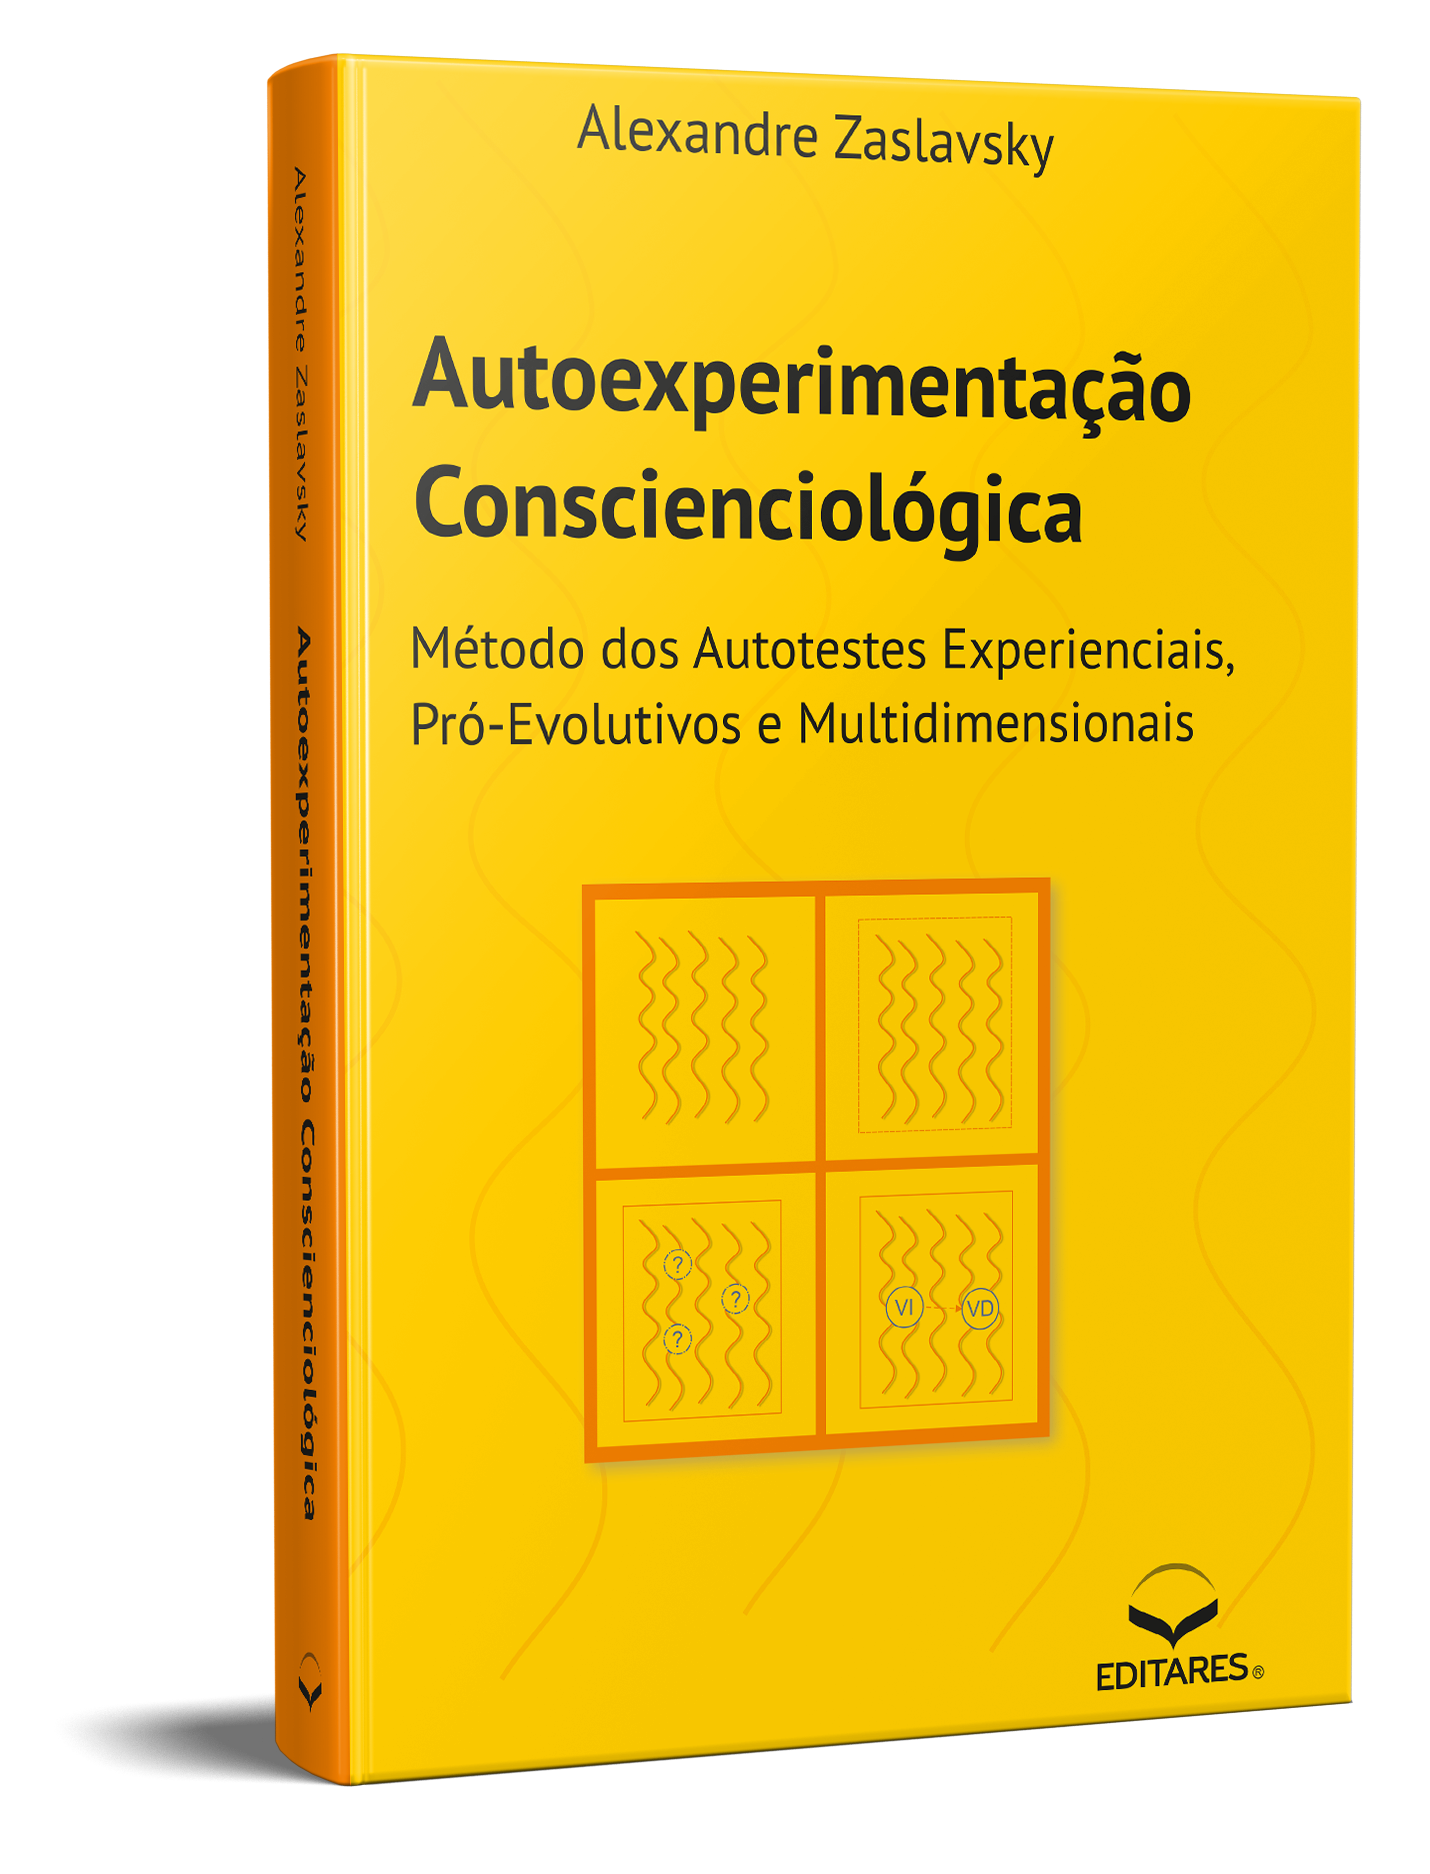
\includegraphics[width=4cm]{articles/entrevista/mockups/Alexandre-Zas.png}
%\end{center}

\textbf{}

\noindent
\includegraphics[width=9cm]{articles/resumo/fotos/materia1/IMG20241023144802.jpg}


No dia 23 de outubro de 2024, a~Editares completou duas décadas de atuação dedicada à~publicação técnico-científica de obras conscienciológicas. Para marcar os 20 anos de existência, a~editora promoveu uma série de atividades comemorativas ao longo da semana, integrando voluntários, autores e~leitores em momentos de reflexão, confraternização e~interassistência.

A programação contou com uma \textbf{semana de verbetes temáticos,} realizada no \emph{Tertuliarium} do CEAEC, com a~participação de autores e~leitores em debates e~apresentações de temas relacionados ao propósito editorial da Editares. Também houve um \textbf{Círculo Mentalsomático temático,} focado na escrita interassistencial e~na importância das publicações para a~expansão da Conscienciologia.

Um dos pontos altos da celebração foi o~\textbf{lançamento do livro ``Interassistência'',} de autoria da voluntária do Conselho Editorial, \textbf{Roberta Bouchardet.} A~obra amplia a~abordagem da assistência multidimensional.

Além das atividades de debate, os voluntários participaram de um \textbf{jantar temático português,} organizado pelo restaurante Primener, no campus do CEAEC. A~noite foi marcada pelo clima de gratidão e~união entre os voluntários da Editares e~convidados.

No dia 23, data oficial do aniversário, a~comemoração seguiu após a~Tertúlia, com \textbf{bolo comemorativo e~momentos de confraternização} entre voluntários, amigos e~apoiadores da Editares, celebrando o~continuísmo do trabalho em equipe e~o~compromisso com a~tarefa esclarecedora.

Com 20 anos de história, a~Editares reafirma seu papel na difusão da Conscienciologia por meio da escrita e~da publicação de obras que promovem o~esclarecimento e~a~evolução das consciências. A~celebração reforçou o~valor da escrita interassistencial ao modo de instrumento de mudança e~continuidade da maxiproéxis grupal.

% {[}COLOCAR ALGUMAS FOTOS{]} As fotos estão na pasta do drive: Matéria 1: Editares celebra 20 anos com programação especial - elas podem ser num tamanho pequeno; aparecer no final ou intercalando com o~texto

%\begin{pullquote}
%``A escrita de uma obra conscienciológica é~uma oportunidade evolutiva inigualável.''
%\end{pullquote}

\noindent
\includegraphics[width=9cm]{articles/resumo/fotos/materia1/IMG20241023143149.jpg}
        
    \end{multicols}
\end{document}

    \documentclass{gescons}

\genre {Resumo do Biênio}
\author{Amanda Vieira}
\title{Editares no XXXVI Congraçamento das ICs: Plaquinhas, sorrisos e escrita}

\begin{document}
    \makeentrevistatitle
    %\maketitle

    %\fullwidthimage{fields}{b}

    %\coverart{back/editorial}
    \coverart{../fundo-generico.png}
    
%    \begin{multicols}{2}

%\begin{center}
%    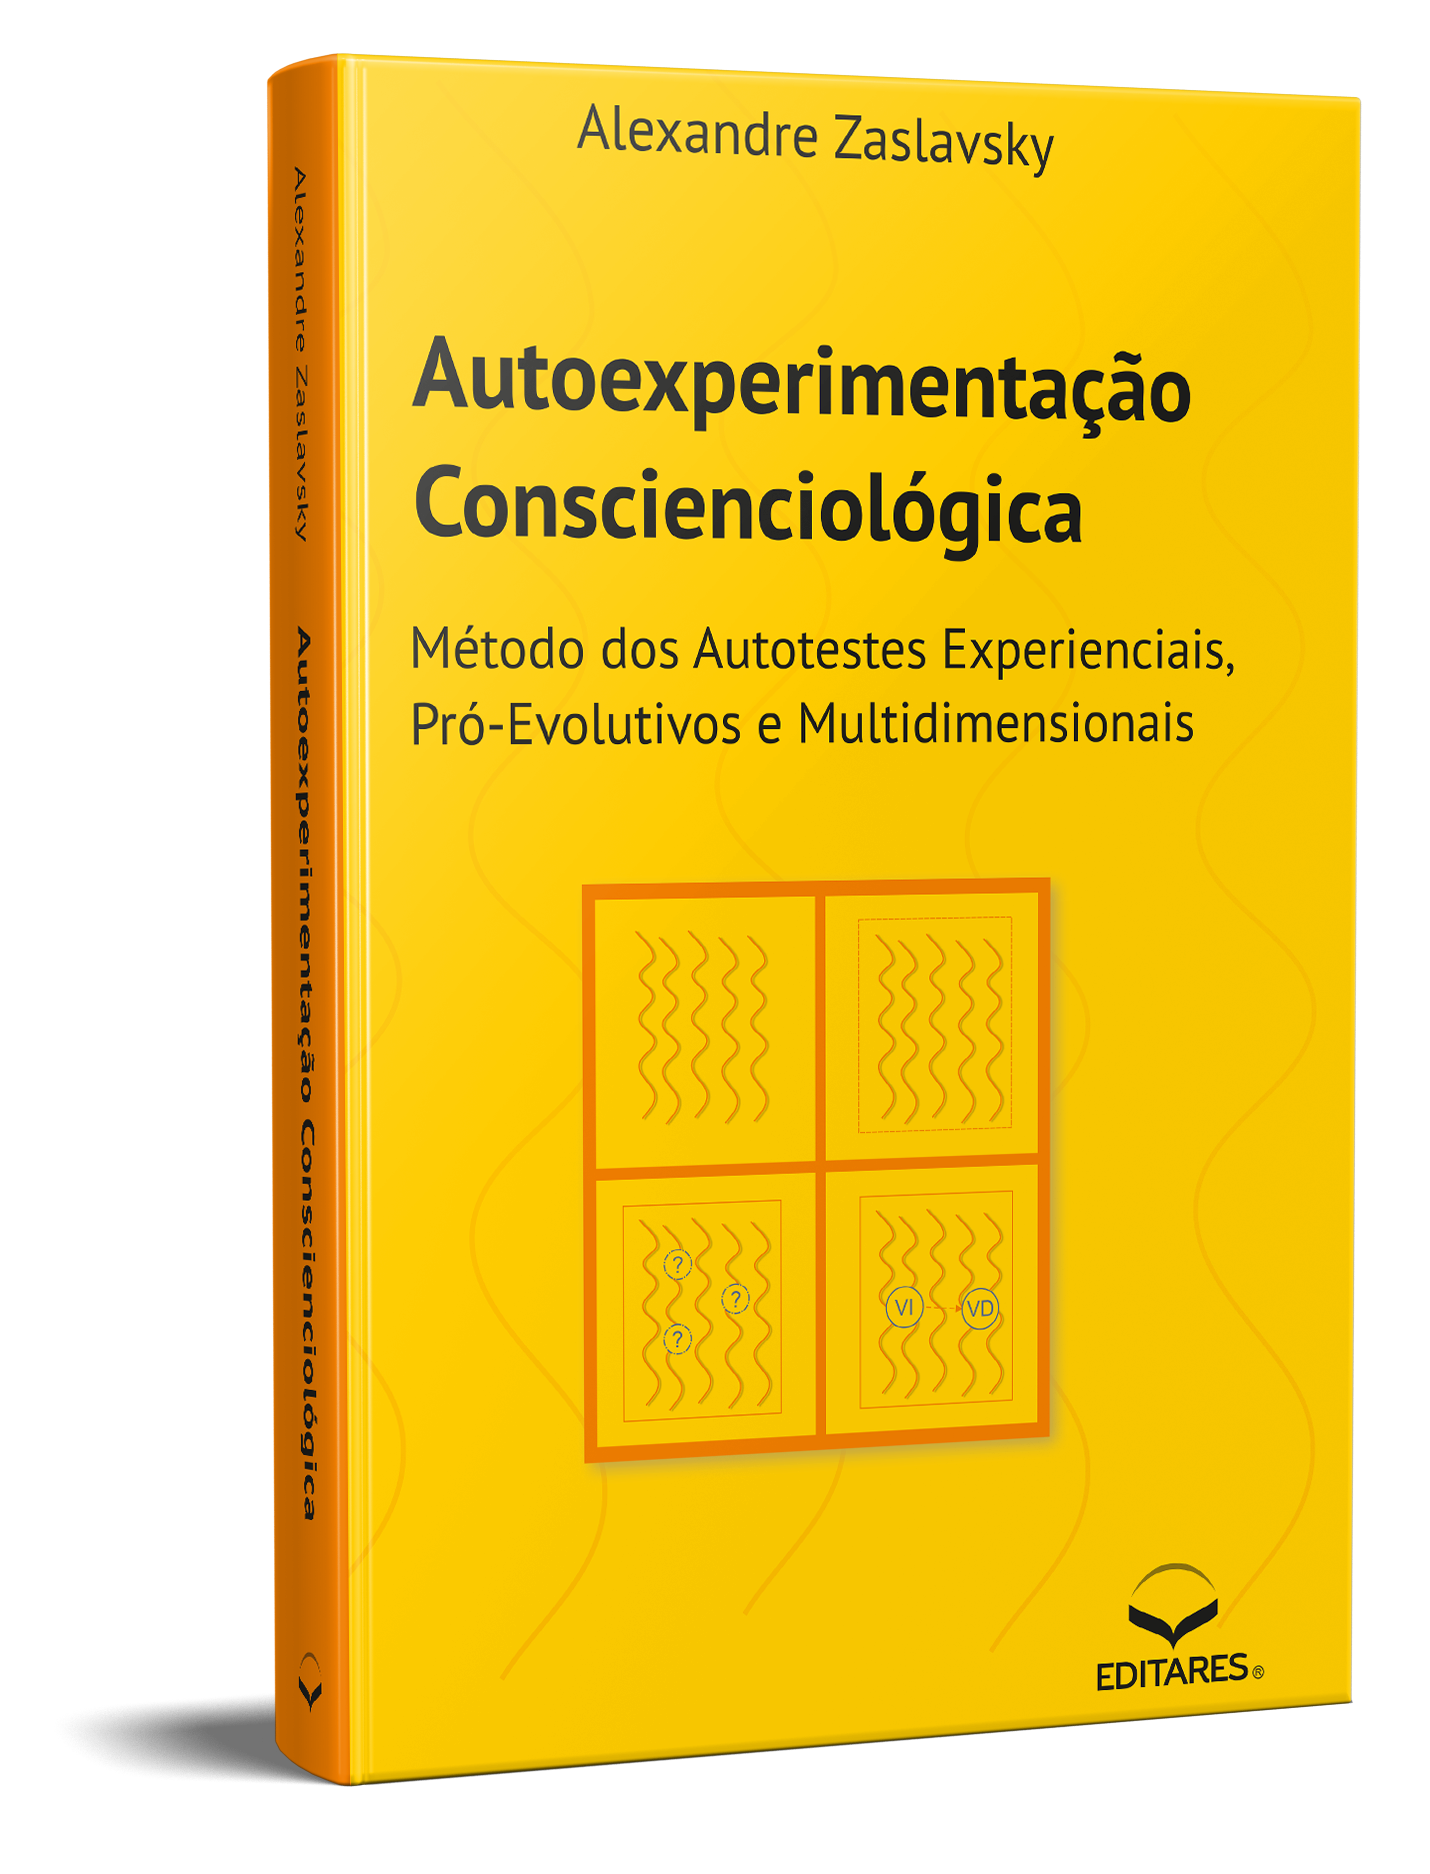
\includegraphics[width=4cm]{articles/entrevista/mockups/Alexandre-Zas.png}
%\end{center}





No dia 8 de dezembro de 2024, durante o tradicional \textbf{Congraçamento das ICs} -- evento anual de celebração do voluntariado conscienciológico --, a Editares marcou presença com uma ação voltada aos \textbf{autores e futuros autores}.

Com placas instigativas e frases de compromisso com a escrita, os voluntários foram convidados a tirar fotos simbolizando o engajamento na tarefa autoral. A atividade trouxe um clima de \textbf{descontração e leveza}, ao mesmo tempo em que reforçou a importância do autoposicionamento proexológico perante a escrita conscienciológica.

\textbf{Confira as fotos!}

  \begin{minipage}[b]{0.32\textwidth}
    
\includegraphics[width=\linewidth]{articles/resumo/fotos/materia2/IMG20241208144202.jpg}
  \end{minipage}\hfill
  \begin{minipage}[b]{0.32\textwidth}
    
\includegraphics[width=\linewidth]{articles/resumo/fotos/materia2/IMG20241208145756.jpg}
  \end{minipage}\hfill
  \begin{minipage}[b]{0.32\textwidth}
    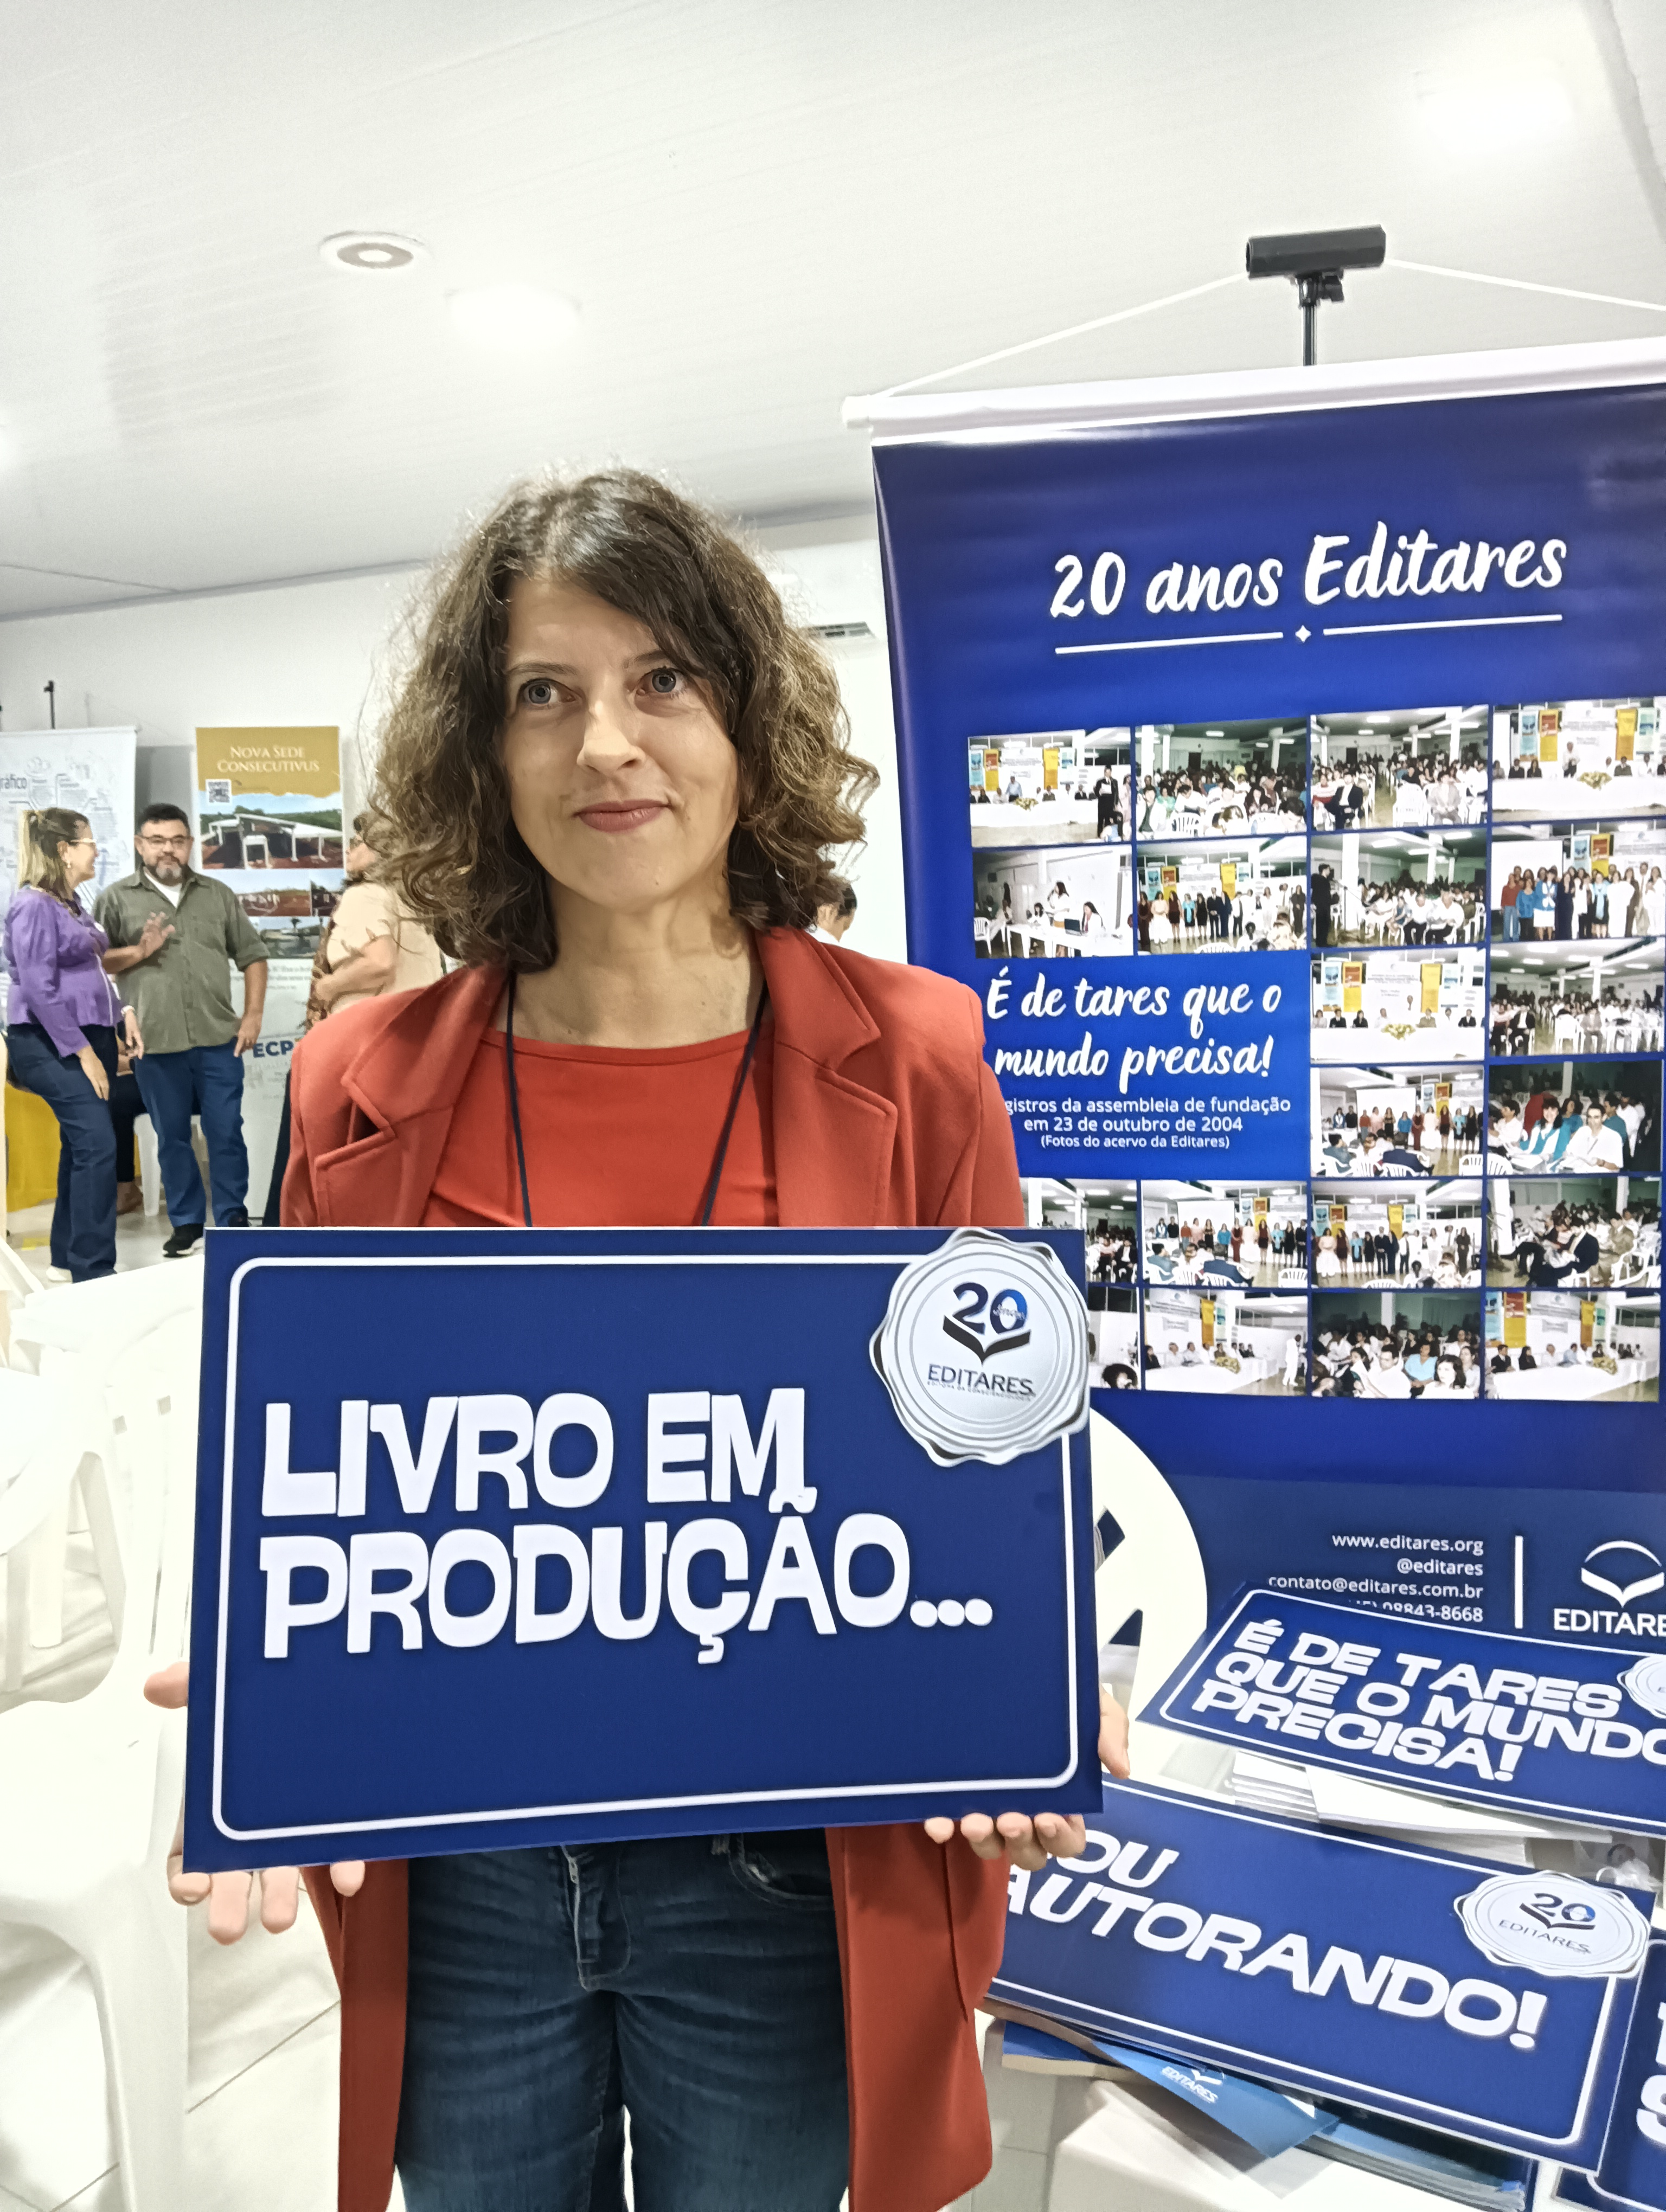
\includegraphics[width=\linewidth]{articles/resumo/fotos/materia2/IMG20241208144514.jpg}
  \end{minipage}
  
  \centering
  \begin{minipage}[b]{0.32\textwidth}
    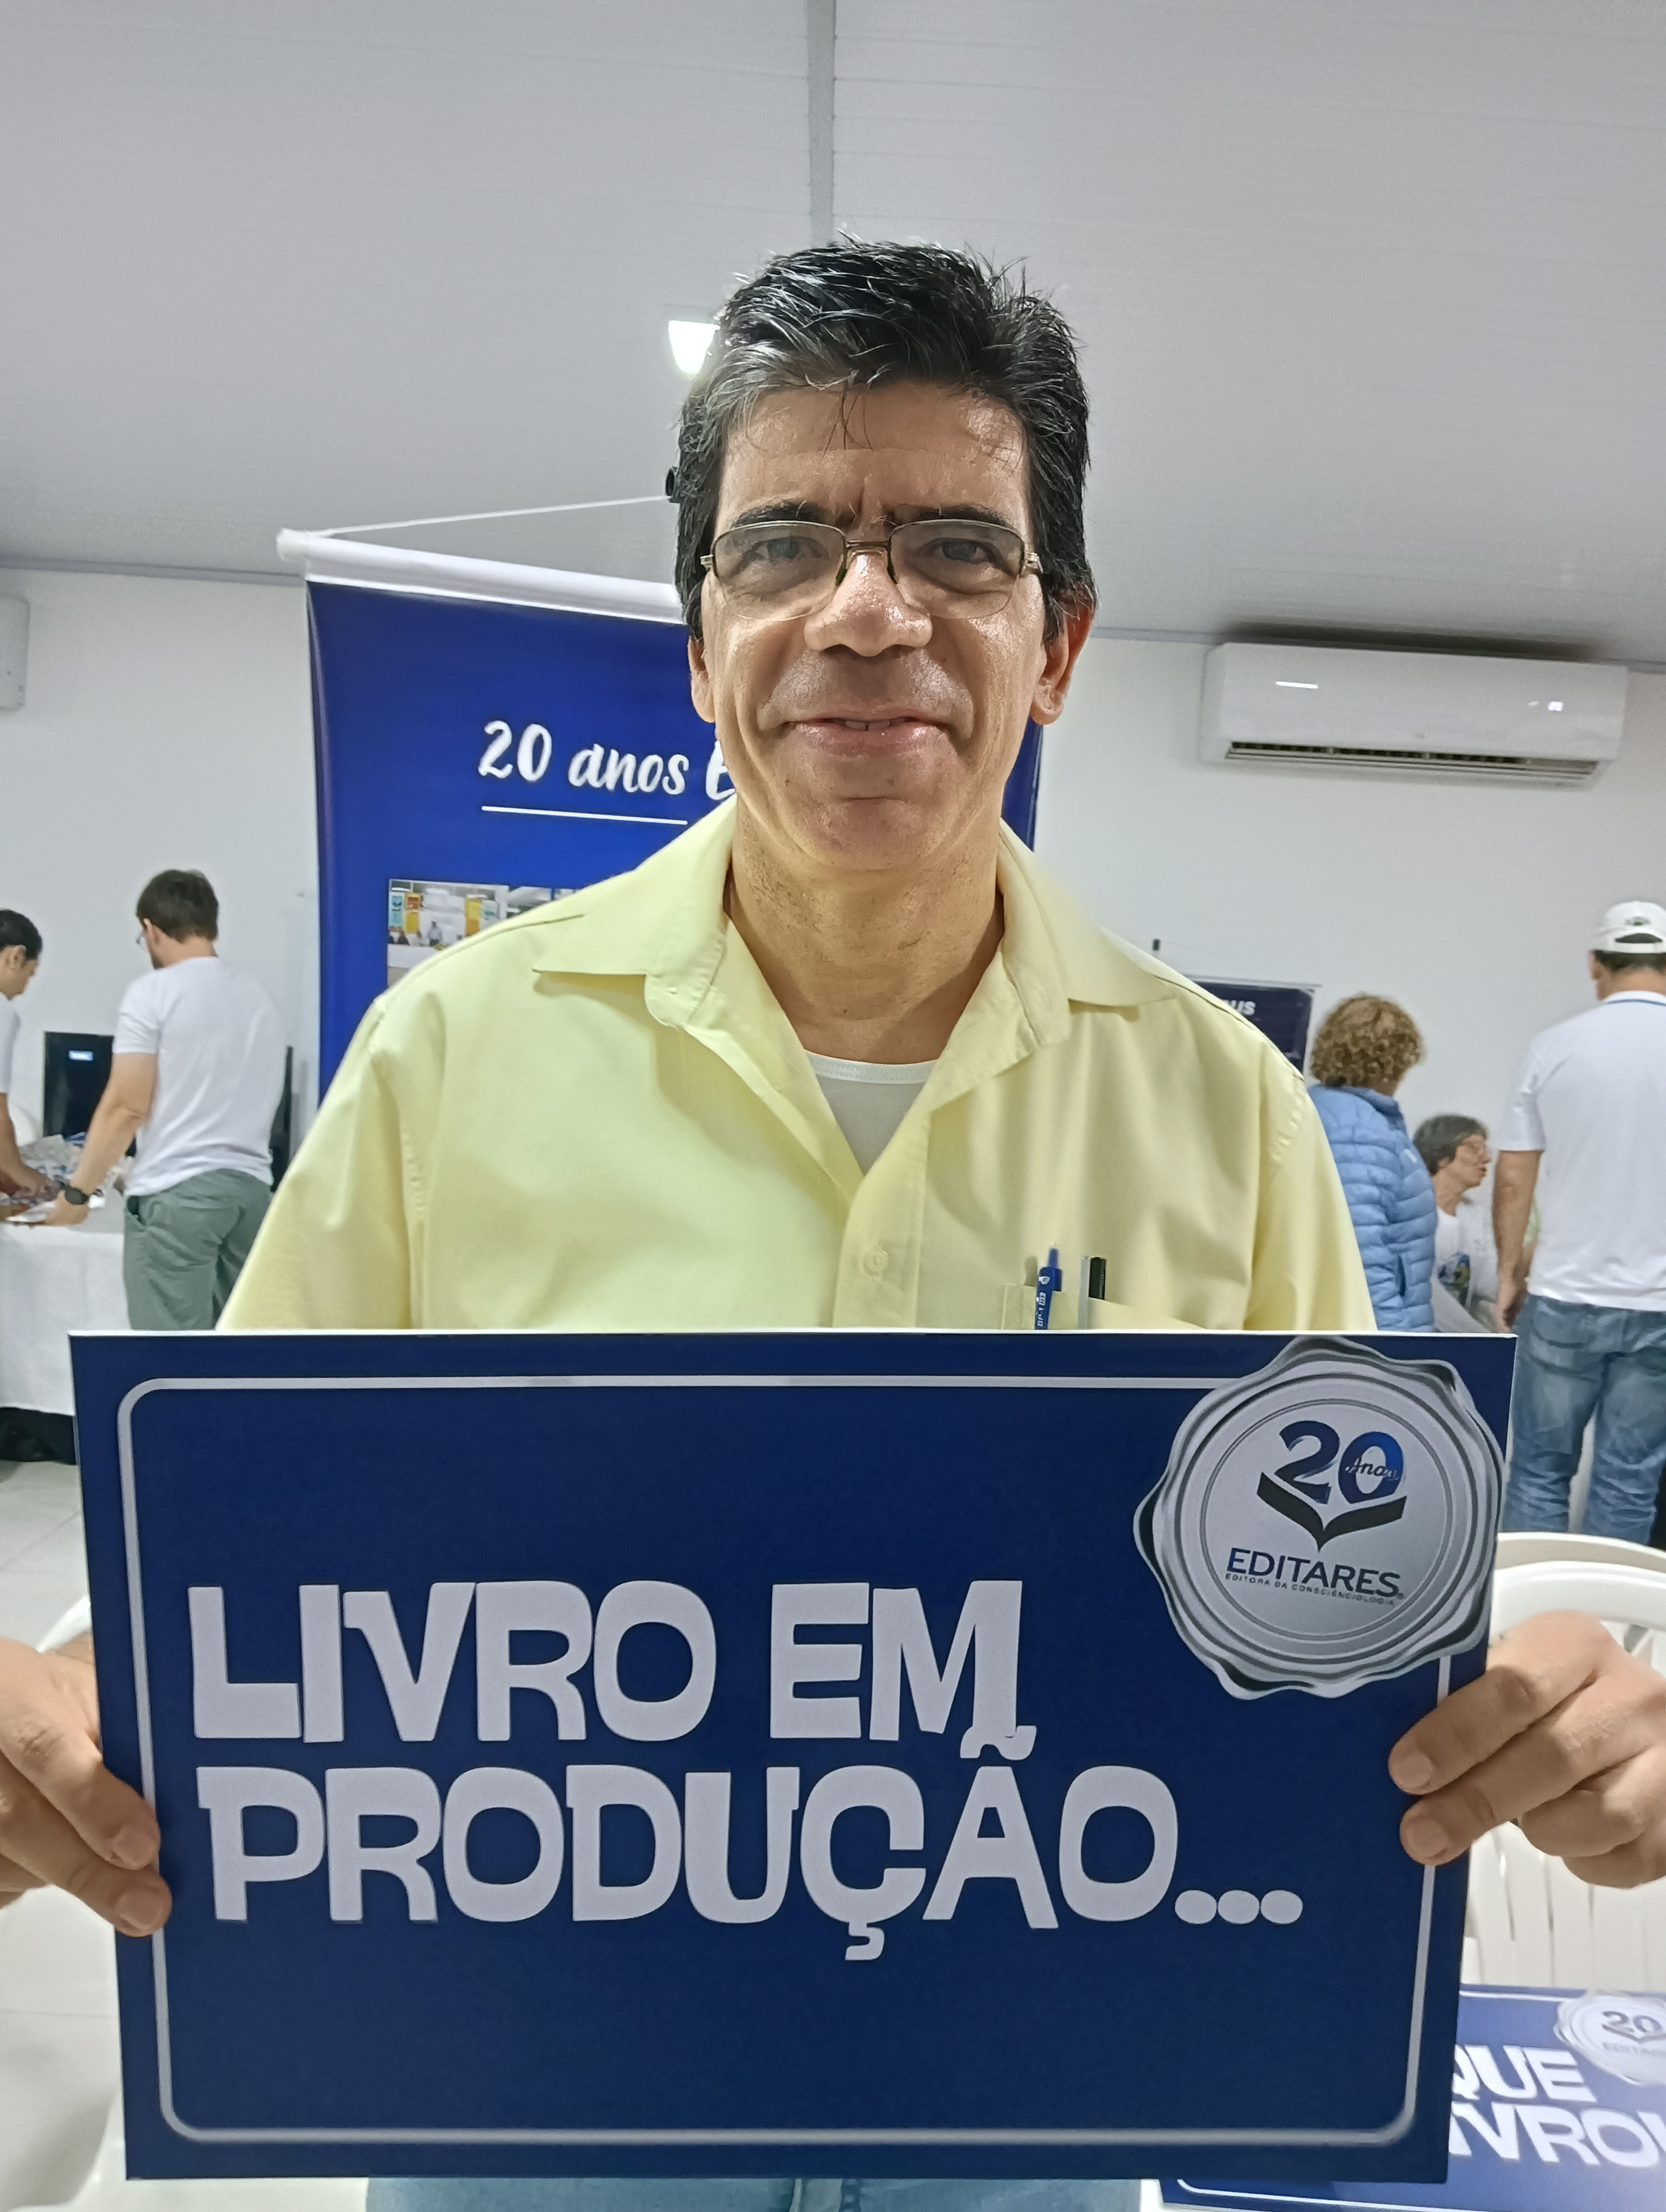
\includegraphics[height=5cm]{articles/resumo/fotos/materia2/IMG20241208144653.jpg}
  \end{minipage}\hfill
  \begin{minipage}[b]{0.55\textwidth}
    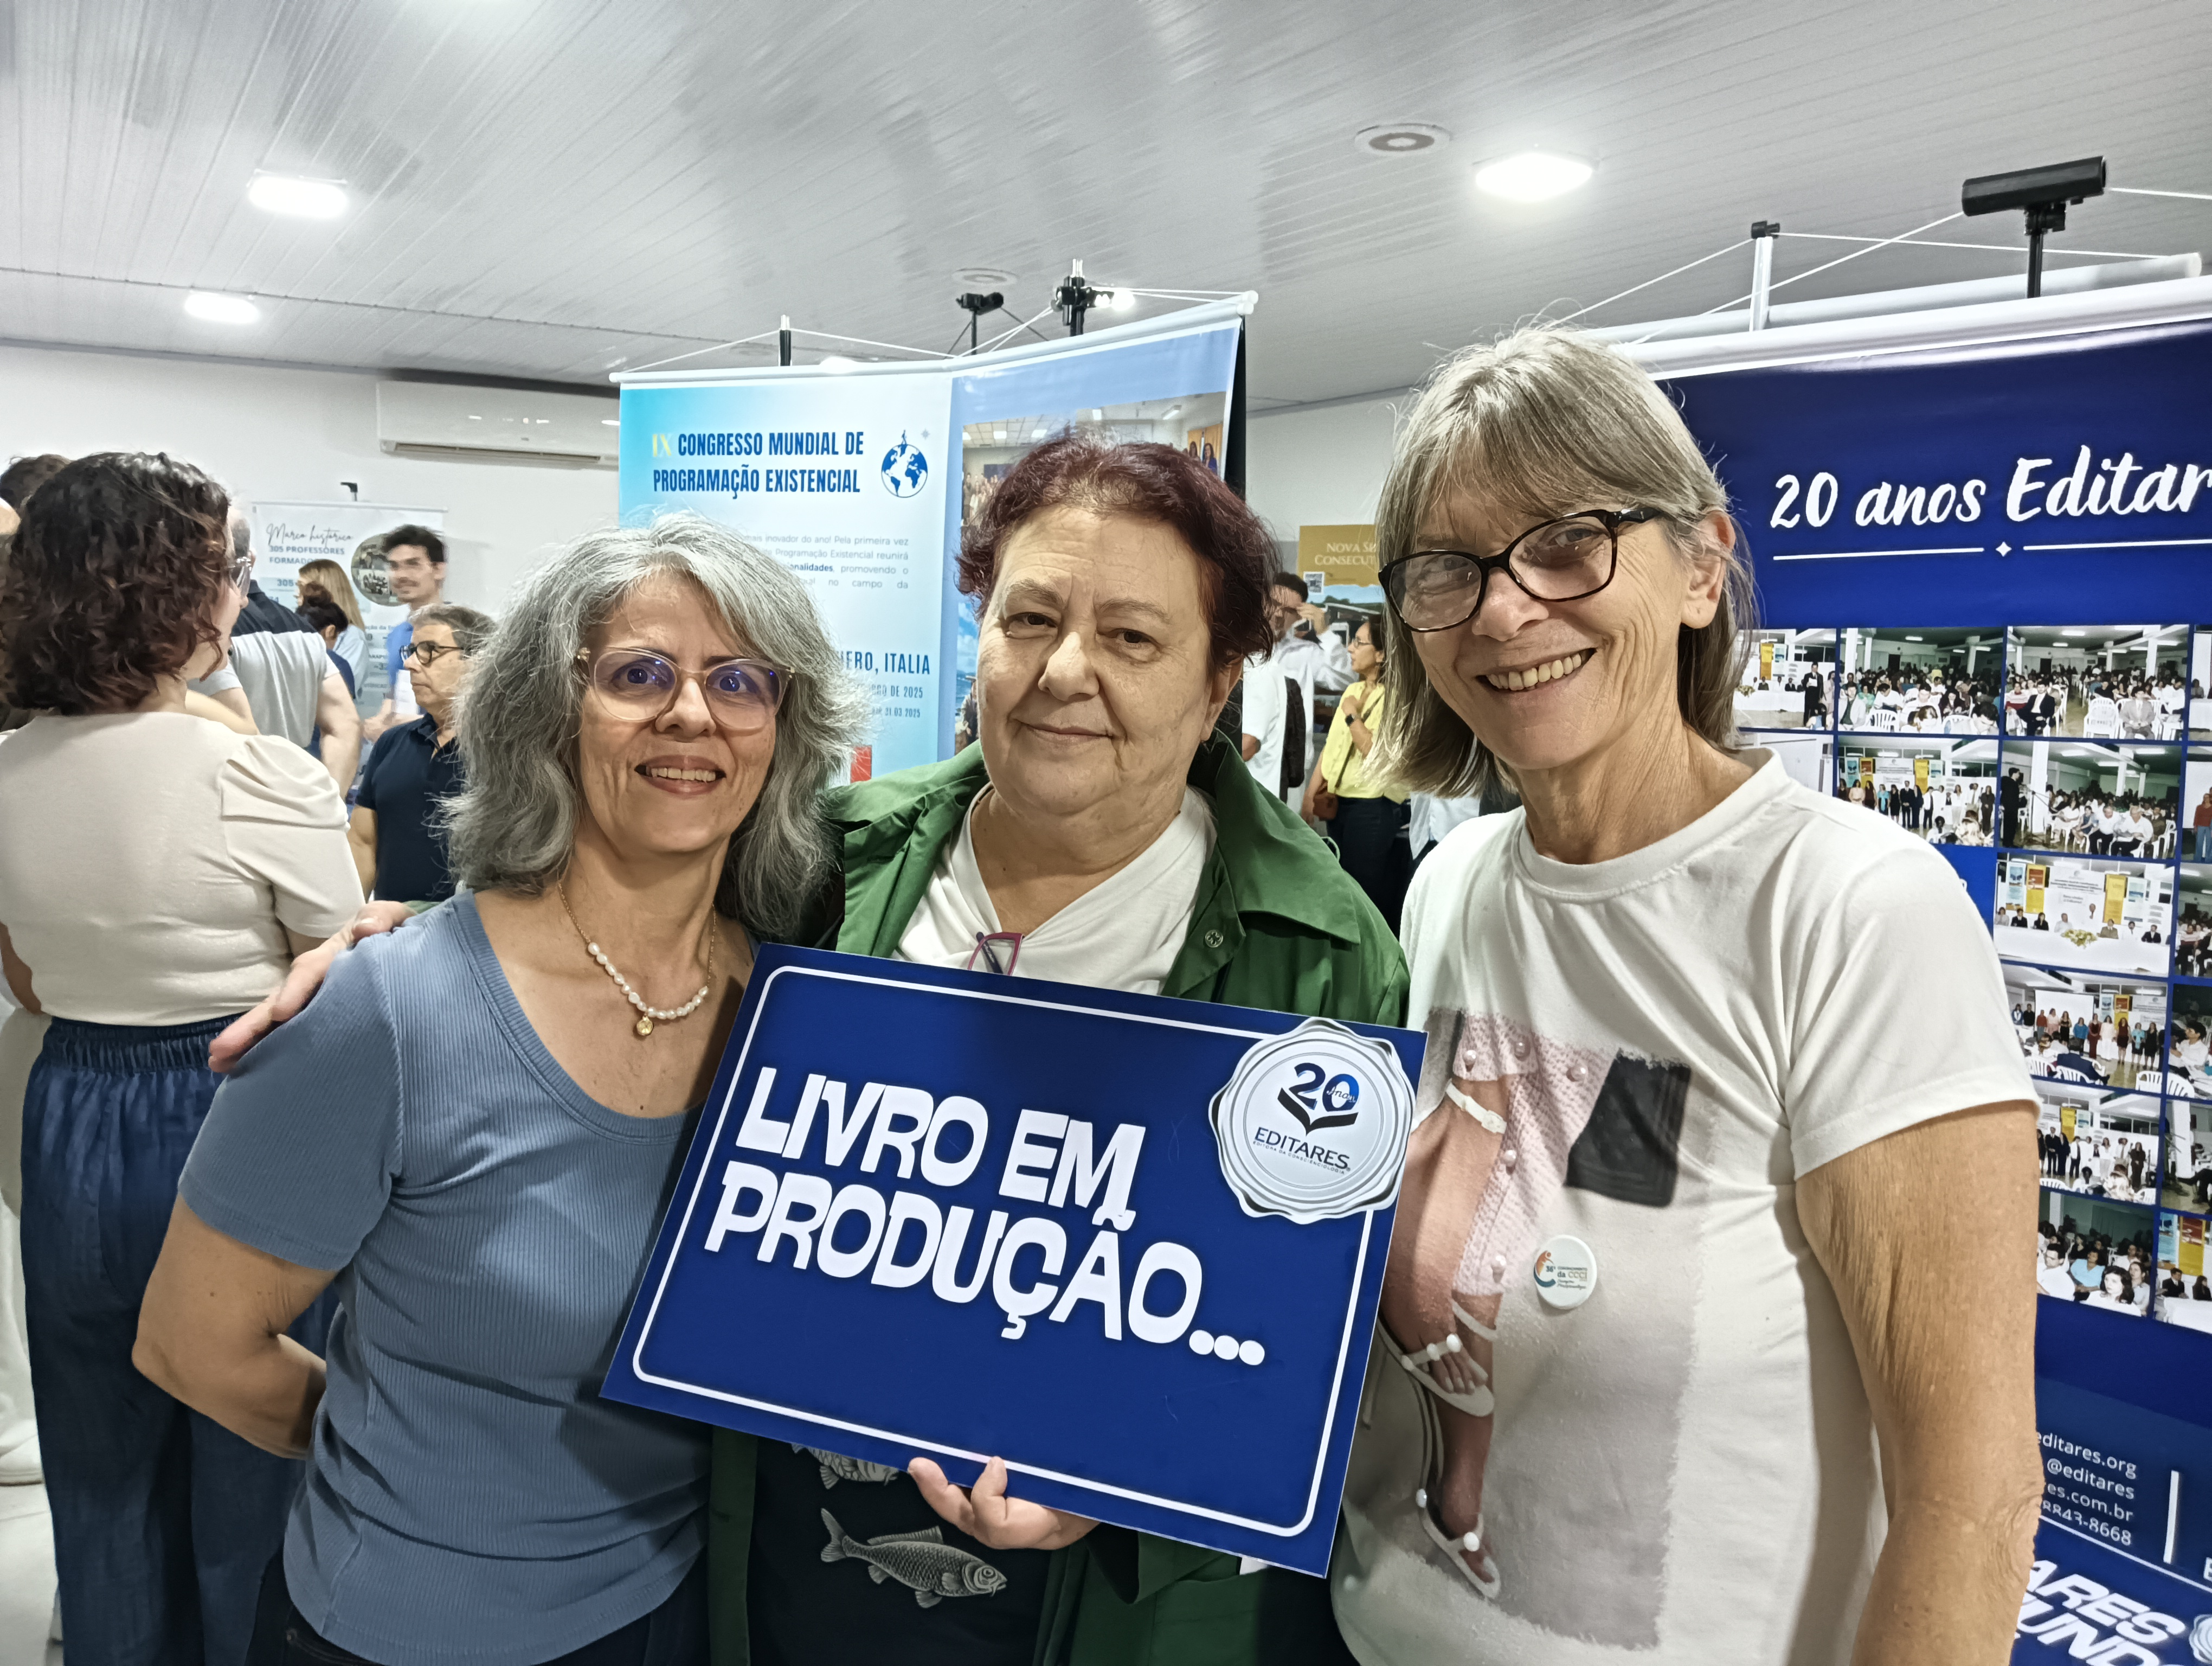
\includegraphics[height=5cm]{articles/resumo/fotos/materia2/IMG20241208155101.jpg}
  \end{minipage}

\coverart{../fundo-generico.png}

%{[}MURAL/MOSAICO DE FOTOS{]} Fotos na pasta matéria 2\ldots{} as fotos podem ocupar 2 páginas



        
%    \end{multicols}
\end{document}

    
    \include{articles/entrevista/alexandre}
    \documentclass{gescons}

\genre {Entrevista}
\author{Ana Mazzonetto}
\title{Retomada de Tarefa: Reencontro com o~Paradever Intermissivo}
\paginaurl{https://www.youtube.com/live/9A6h__c2uxk}

\begin{document}
    \makeentrevistatitle

\coverart{back/ana_mazzonetto}

    \begin{multicols}{2}


\begin{center}
%\noindent\includegraphics[width=8cm, height=10cm]{example-image}

    
\includegraphics[width=8cm]{articles/entrevista/mockups/Ana-Mazzonetto}
\end{center}

\subsubsection{1. Qual foi a~motivação para a~escrita da obra? Por que a~definição deste tema para publicação de um livro?}

O livro é~fruto de demanda extrafísica, portanto a~maior motivação foi o~próprio convite mesmo. 

Desde o~ano de 2020, o~foco pesquisístico estava voltado ao tema do “antiassoberbamento”. Estava em curso projeto para a~escrita de livro sobre o~tema. Todavia, em 10 de julho de 2022, após a~conclusão da técnica da tenepes, sobreveio convite, por parte de amparadores extrafísicos, para a~escrita e~publicação de livro conscienciológico acerca da retomada de tarefa. 

A clareza da demanda extrafísica não deixou dúvidas sobre a~importância do tema. Desde então, a~pesquisa e~a~produção gesconográfica voltaram-se ao entendimento teático da temática.

\subsubsection{2. Quais foram as principais percepções, intra e~extrafísicas, durante a~pesquisa e~a~escrita da obra? E~posterior ao lançamento?}

Durante a~escrita da obra, vivenciei muitos acoplamentos mentaissomáticos com os amparadores, tanto nas fases de escrita, quanto de pesquisa, formulação de hipóteses e~reflexões plasmadas no livro. 

Parecia que tudo que enxergava tinha relação com a~temática, foi experiência muito legal de hiperfoco. Verifiquei também o~aumento gradativo do público-alvo interassistencial.

Após o~lançamento, a~principal percepção foi de aumento da responsabilidade interassistencial. 

\subsubsection{3. Qual o~maior aprendizado com a~escrita desta obra?}

Aprendi a~valorizar meus trafores, sem eles o~livro não teria saído do campo das ideias. Compreendi também o~alcance interassistencial da autaceitação da história pessoal.

\begin{pullquote}
``Compreendi também o~alcance interassistencial da autaceitação da história pessoal''
\end{pullquote}


\subsubsection{4. O~que poderia dizer como incentivo para que mais pesquisadores invistam na publicação de obras conscienciológicas?}

Escolha o~tema de seu livro, invista na qualificação recinológica e~gesconográfica e~só pare quando o~livro estiver pronto, simples assim. 

Ouse escrever, intermissivista!

\begin{pullquote}
``Escolha o~tema de seu livro, invista na qualificação recinológica e~gesconográfica e~só pare quando o~livro estiver pronto, simples assim.''
\end{pullquote}



    
    \end{multicols}
\end{document}

    \documentclass{gescons}

\genre {Entrevista}
\author{Cristina Bassanesi}
\title{O Calidoscópio da Evolução Consciencial: Abordagem Interparadigmática da Evoluciologia}


\begin{document}
    \makeentrevistatitle
    \coverart{back/Cristina_Bassanesi}

    \begin{multicols}{2}

\textbf{Qual foi a motivação para a escrita da obra? Por que a definição deste tema para publicação de um livro?}

Esta obra teve como motivação escrever sobre a \textit{Mutabilidade Consciencial Não Linear,} tema pertinente à \textit{Especialidade Evoluciologia,} empregando abordagem científica, multidisciplinar e interparadigmática.

A definição pelo tema somente foi estabelecida em definitivo após o movimento pessoal de começar a escrever. O roteiro previamente delineado mudou logo no início, quando ampliei a cosmovisão sobre o que poderia ser o tema central do livro e passei a aplicar \textit{o princípio de os fatos e parafatos orientarem a pesquisa.}

\textbf{Quais foram as principais percepções, intra e extrafísicas, durante a pesquisa e a escrita da obra? E posterior ao lançamento?}

Atitude pessoal determinante para manter a rotina de escrita foi o autoposicionamento de priorizar 1 turno fixo do dia (manhã) para à escrita, em detrimento dos inúmeros apelos para envolvimento em outras atividades. Nesse ponto, a sobreveniência do desassédio mentalsomático e a parapercepção do amparo de função, atuando tanto com inspirações quanto no auxílio à resolução de entraves dos mais variados tipos tornou-se evidente.

As repercussões favoráveis do livro publicado trouxeram grande alegria, porém, com maior intensidade, asseveraram o autocompromisso intermissivo com a tares autoral. 

\begin{pullquote}
``As repercussões favoráveis do livro publicado trouxeram grande alegria, porém, com maior intensidade, asseveraram o autocompromisso intermissivo com a tares autoral.''
\end{pullquote}

\textbf{Qual o maior aprendizado com a escrita desta obra?}

Sem dúvida, a conclusão da obra deixou saldo de aprendizados, dentre os quais destaco o valor do exercício da persistência e paciência na sustentação gesconográfica. Aprendizado adicional foi o de eliminar o apego a ideias, frases e até vocábulos, que a princípio podem soar muito boas. Contudo, por vezes, atravancam durante horas ou dias a fluidez da escrita. A sugestão é guardá-las em algum arquivo próprio, para utilização em outra oportunidade. 

\begin{pullquote}
``Sem dúvida, a conclusão da obra deixou saldo de aprendizados, dentre os quais destaco o valor do exercício da persistência e paciência na sustentação gesconográfica.''
\end{pullquote}

\textbf{O que poderia dizer como incentivo para que mais pesquisadores invistam na publicação de obras conscienciológicas?}

Deixo o incentivo, aos potenciais escritores, a investirem na escrita de obras conscienciológicas, expondo as autossingularidades ou especialidades pessoais, as quais podem trazer novos vieses de compreensão sobre a evolução consciencial e novas senhas aos neointermissivistas. 

    %\noindent\includegraphics[width=11cm, height=12cm]{example-image} 

\begin{center}
    \includegraphics[width=8cm]{articles/entrevista/mockups/Cristina-Bassanesi.png}
    %\noindent\includegraphics[width=8cm, height=10cm]{example-image}
\end{center}
    
    \end{multicols}
\end{document}

    \documentclass{gescons}

\genre {Entrevista}
\author{Daniel Mamede}
\title{Ações Antifanatismo: Intensidade Lúcida em Autopesquisas e Autorreciclagens}

\begin{document}
    \makeentrevistatitle

    \coverart{back/Daniel-Mamede}
    \begin{multicols}{2}

\begin{center}
    
\includegraphics[width=8cm]{articles/entrevista/mockups/Daniel-Mamede.png}
\end{center}

%\noindent\includegraphics[width=9cm, height=10cm]{example-image} 

\textbf{1. Qual foi a motivação para a escrita da obra? Por que a definição deste tema para publicação de um livro?}

O livro “Ações Antifanatismo” representa muito para mim, por ter sido o resumo dos meus 10 primeiros anos de contato e vivência do paradigma consciencial. 

Escrito em princípio para mim mesmo, para poder organizar, reeducar e curar aspectos negativos das automanifestações, muitas delas tendentes ou vinculadas ao fanatismo, o livro mostrou \textit{a vida teática no papel,} isto é, materializou, grafou e vincou a autopesquisa conscienciológica sendo vivenciada dia a dia, pensene a pensene, aprendizado a aprendizado, resultando em material com enorme potencial para ajudar outras pessoas que possam estar em apuros com o mesmo assunto, notadamente os intermissivistas, os quais partilham de propósitos e objetivos similares aos meus para esta vida humana.



\textbf{2. Quais foram as principais percepções, intra e extrafísicas, durante a pesquisa e a escrita da obra? E posterior ao lançamento?}

O que este livro mais tem são percepções e parapercepções vivenciadas durante os processos de reciclagem, pois seu estilo de escrita predominante foi o do “\textit{in media res}”, isto é, as experiências da vida eram grafadas e autocriticadas de modo praticamente concomitante às ocorrências. Vale muito a pena conferir. 


\textbf{3.       Qual o maior aprendizado com a escrita desta obra?}

Nos últimos 10 anos, nunca deixei passar mais que 24 horas entre o intervalo da ocorrência dos fatos ou parafatos e as devidas anotações. Por isso, o efeito das vivências descritas no livro traz as energias dos momentos das aprendizagens disruptivas de modo bastante intenso e real. E essa rotina continua firme na minha vida, mesmo após a conclusão do livro, pois a autopesquisa conscienciológica nunca pode parar. Este foi meu maior aprendizado ao ver o livro concluído.

\begin{pullquote}
``O efeito das vivências descritas no livro traz as energias dos momentos das aprendizagens disruptivas de modo bastante intenso e real.''
\end{pullquote}


\textbf{4.       O que poderiam dizer como incentivo para que mais pesquisadores invistam na publicação de obras conscienciológicas?}

Fazer autopesquisas diárias e comprometidas como as descritas em “Ações Antifanatismo” é um dos caminhos mais tranquilos para quem quiser publicar algum livro. Ele vai acontecer naturalmente. Vai estar pronto antes mesmo de o autor o conceber. Foi assim comigo. O acúmulo dos pensenes materializados no papel gerou banco de dados rico e vasto para eu poder explorá-lo da maneira que entendesse por bem, e assim o fiz justamente para trabalhar os traços de temperamento que entendi serem os mais sérios e prioritários em meus processos de reciclagem, no caso, vinculados às posturas fanáticas. Aí, foi só organizar. A rigor, o que direcionou e conduziu a escrita do livro não foi a atenção ao traf\textit{a}r do fanatismo, mas sim ao traf\textit{o}r da valorização e do comprometimento com a ininterruptibilidade da autopesquisa conscienciológica.


    
    
    \end{multicols}
\end{document}

    \documentclass{gescons}

\genre {Entrevista}
\author{Karine Brito}
\title{Gratidão: Reconhecer, Expressar e~Retribuir}
\paginaurl{https://www.youtube.com/live/RN8tWr7Vk3c}

\begin{document}
    \makeentrevistatitle
    \coverart{back/Karine_Brito}

    \begin{multicols}{2}

\begin{center}
    
\includegraphics[width=8cm]{articles/entrevista/mockups/Karine-Brito.png}
\end{center}

\textbf{1. Qual foi a~motivação para a~escrita da obra? Por que a~definição deste tema para publicação de um livro?}

A motivação para a~escrita do livro \textit{Gratidão: Reconhecer, Expressar e~Retribuir} foi a~descoberta de uma questão de saúde congênita em 2008, suscitando uma série de autorreflexões sobre a~vida, os vínculos conscienciais nutridos até então e,~sobretudo, o~subnível evolutivo quanto à~programação existencial.  A~doença foi um alerta consciencial para ampliar o~autodiscernimento, possibilitando identificar um grande travão evolutivo: a~ingratidão. A~escrita do livro surgiu como uma forma de retribuição lúcida das inúmeras benesses recebidas nesse processo. A~inspiração extrafísica era explicitar como se dá o~desenvolvimento da cognição sobre a~gratidão, incentivando o~seu cultivo autoconsciente no dia a~dia. 

\begin{pullquote}
``A doença foi um alerta consciencial para ampliar o~autodiscernimento, possibilitando identificar um grande travão evolutivo: a~ingratidão.''
\end{pullquote}

\textbf{2. Quais foram as principais percepções, intra e~extrafísicas, durante a~pesquisa e~a~escrita da obra? E~posterior ao lançamento?}

Ao longo dos 16 anos de pesquisa e~escrita desta obra percebi de modo ostensivo a~atuação dos amparadores, intra e~extrafísicos. Muitos amigos evolutivos acompanharam de perto o~desenvolvimento da pesquisa, ajudando nas autorreflexões, nos debates sobre o~tema e~nas revisões. Durante a~escrita do livro, desde o~início tive muitas inspirações da equipex. Percebia um interesse genuíno dos amparadores em materializar esta publicação, destacando a~sua relevância no momento evolutivo atual. A~principal inspiração extrafísica foi apresentar, de modo técnico e~didático, a~gratidão como base da recomposição grupocármica. Posterior ao lançamento, me chamou a~atenção a~assistência a~ouvintes de curso intermissivo ligados à~invéxis, muito atentos ao tema da gratidão.

\begin{pullquote}
``Percebia um interesse genuíno dos amparadores em materializar esta publicação, destacando a~sua relevância no momento evolutivo atual.''
\end{pullquote}

\textbf{3. Qual o~maior aprendizado com a~escrita desta obra?}

O maior aprendizado com a~escrita desta obra foi, sem dúvida, levar a~sério o~alerta consciencial proexológico, colocando a~recomposição grupocármica como prioridade. Isso foi a~mola propulsora evolutiva para desenvolver a~gratidão. 

\textbf{4. O~que poderia dizer como incentivo para que mais pesquisadores invistam na publicação de obras conscienciológicas?}

A obra conscienciológica é~retribuição fundamental do intermissivista, favorecendo o~autorrevezamento lúcido e~a~ampliação da interassistencialidade tarística a~partir da recin do autor. Se você melhorou, ajude outras pessoas a~chegarem até lá! 
    
    
    \end{multicols}
\end{document}




    \documentclass{gescons}

\genre {Entrevista}
\author{Ana Luiza Rezende e~Mabel Teles}
\authorrole{Organizadoras}
\title{Epicentrismo Consciencial: Casuísticas Recinológicas}
\paginaurl{https://www.youtube.com/live/yFrO2lGJzFo}

\begin{document}
    \makeentrevistatitle
    \coverart{back/Mabel_Teles_Ana_Luiza_Rezende}

    \begin{multicols}{2}

%\noindent\includegraphics[width=9cm, height=10cm]{example-image} 

\begin{center}
    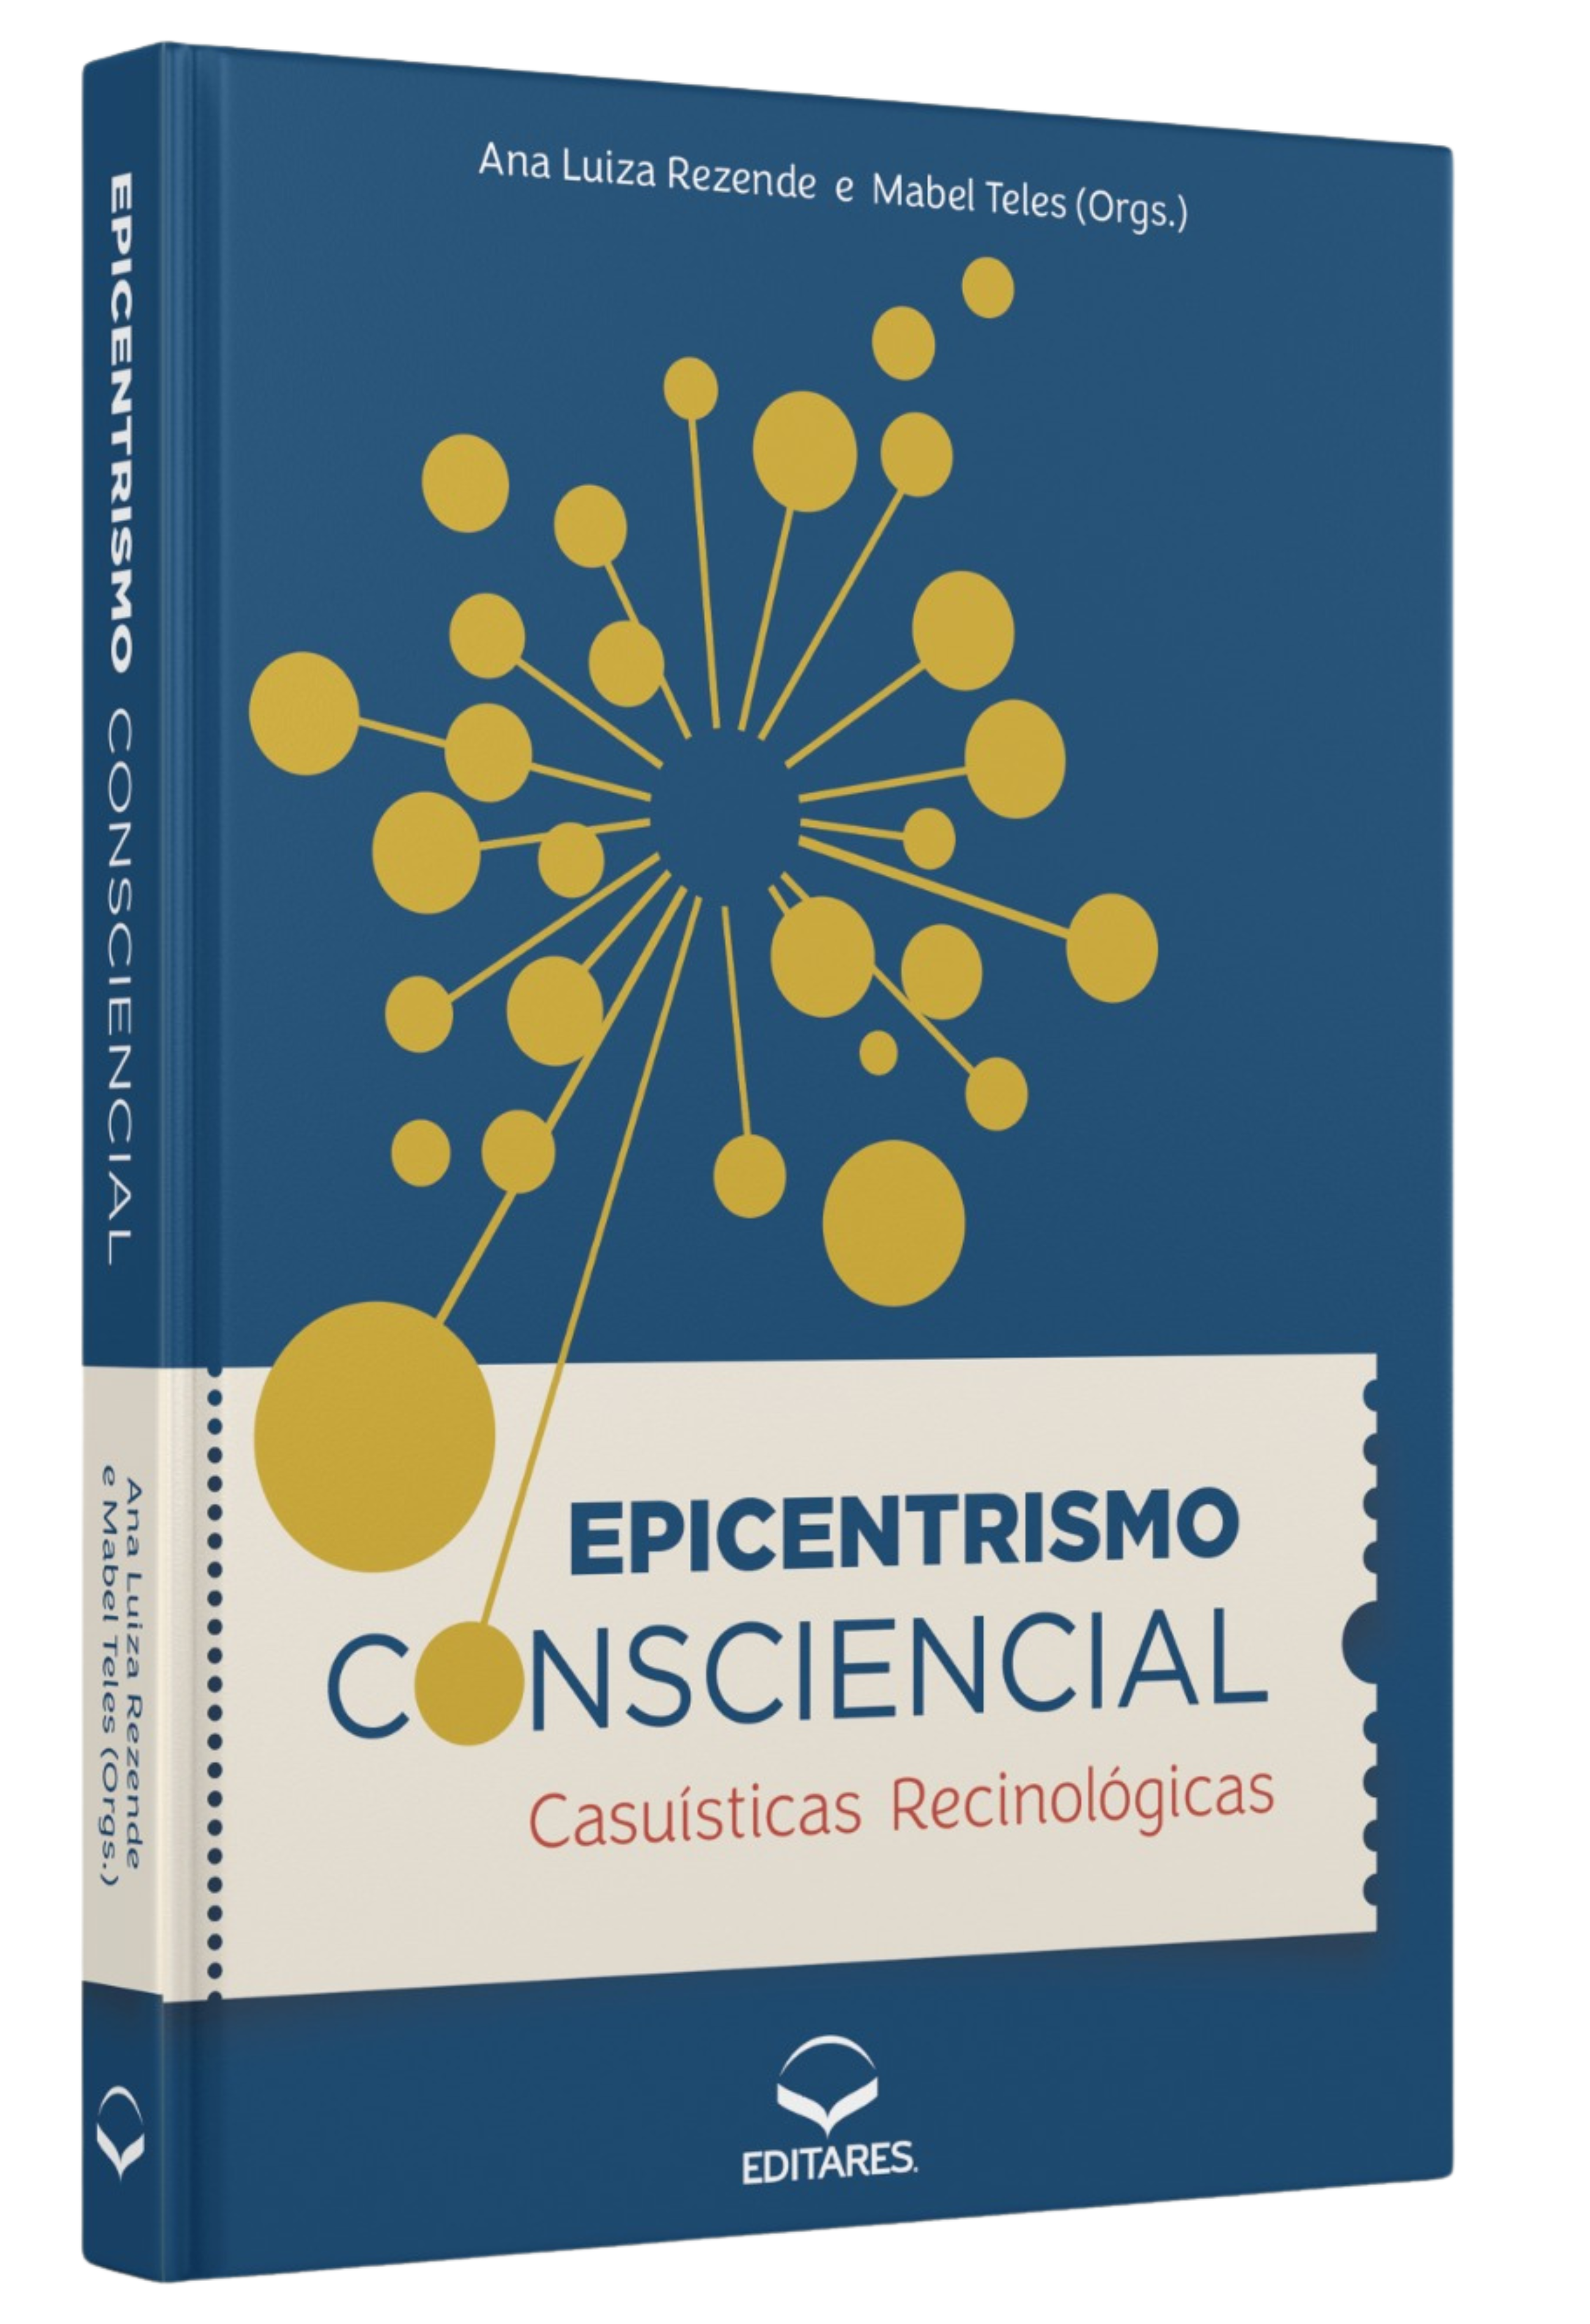
\includegraphics[width=8cm]{articles/entrevista/mockups/Mabel-e-Ana-Luiza.png}
\end{center}

\subsubsection{1. Qual foi a~motivação para a~escrita da obra? Por que a~definição deste tema para publicação de um livro?}


O livro \textit{Epicentrismo Consciencial – Casuísticas Recinológicas} surgiu a~partir de uma sugestão do Prof. Waldo Vieira (1932--2015), em reunião do \textit{Conselho de Epicons} (CE), realizada no \textit{Hotel Interludium,} Foz do Iguaçu, em 2015. Na ocasião, ele propôs um levantamento das recins e~recéxis positivas e~exemplaristas já implementadas pelos integrantes do CE. A~obra é~fruto dessa proposta e~busca responder à~questão levantada no encontro: \textit{quais atos vêm qualificando o~epicentrismo de cada integrante do CE até agora? }

\subsubsection{2. Quais foram as principais percepções, intra e~extrafísicas, durante a~pesquisa e~a~escrita da obra? E~posterior ao lançamento?}

A obra, de cunho biográfico, possibilitou o~resgate de vivências significativas que contribuíram para o~desenvolvimento do epicentrismo de cada autor. O~registro de acertos e~reciclagens permitiu a~identificação de padrões evolutivos pessoais, fortalecendo a~responsabilidade perante a~grupalidade e~a~interassistência. A~publicação tem incentivado pesquisadores conscienciológicos a~aprofundarem as próprias reciclagens, visando à~qualificação do autepicentrismo e~o~aprimoramento da assistência multidimensional.  

\begin{pullquote}
``A obra, de cunha biográfico, possibilitou o~resgate de vivências significativas que contribuíram para o~desenvolvimento do epicentrismo de cada autor.''
\end{pullquote}


\subsubsection{3. Qual o~maior aprendizado com a~escrita desta obra?}

A escrita da obra permitiu o~aprofundamento da autopesquisas, além de ter demonstrado a~relevância da grupalidade na evolução pessoal, destacando como as interações, os desafios e~os aprendizados coletivos fortalecem o~epicentrismo de cada um. 


\subsubsection{4. O~que poderiam dizer como incentivo para que mais pesquisadores invistam na publicação de obras conscienciológicas?}

Publicar obras conscienciológicas é~uma forma de aprofundar a~autopesquisa, consolidar a~cognição evolutiva e~expandir a~interassistência. O~registro das experiências cria um legado evolutivo, beneficiando tanto o~autor quanto os leitores. Além disso, fortalece a~rede de pesquisadores e~contribui para a~ampliação do paradigma consciencial, estimulando novas reflexões e~descobertas.


\begin{pullquote}
``Publicar obras conscienciológicas é~uma forma de aprofundar a~autopesquisa, consolidar a~cognição evolutiva e~expandir a~interassistência.''
\end{pullquote}




    \end{multicols}
\end{document}
















    \documentclass{gescons}

\genre {Entrevista}
\author{Michel Chad}
\title{Megapensenes Trivocabulares Pró-evolutivos}
\paginaurl{https://www.youtube.com/live/lyb7pNbQWh0}

\begin{document}
    \makeentrevistatitle
    \coverart{back/Michel_Chad}

    \begin{multicols}{2}


%\noindent\includegraphics[width=9cm, height=7cm]{example-image} 

\begin{center}
    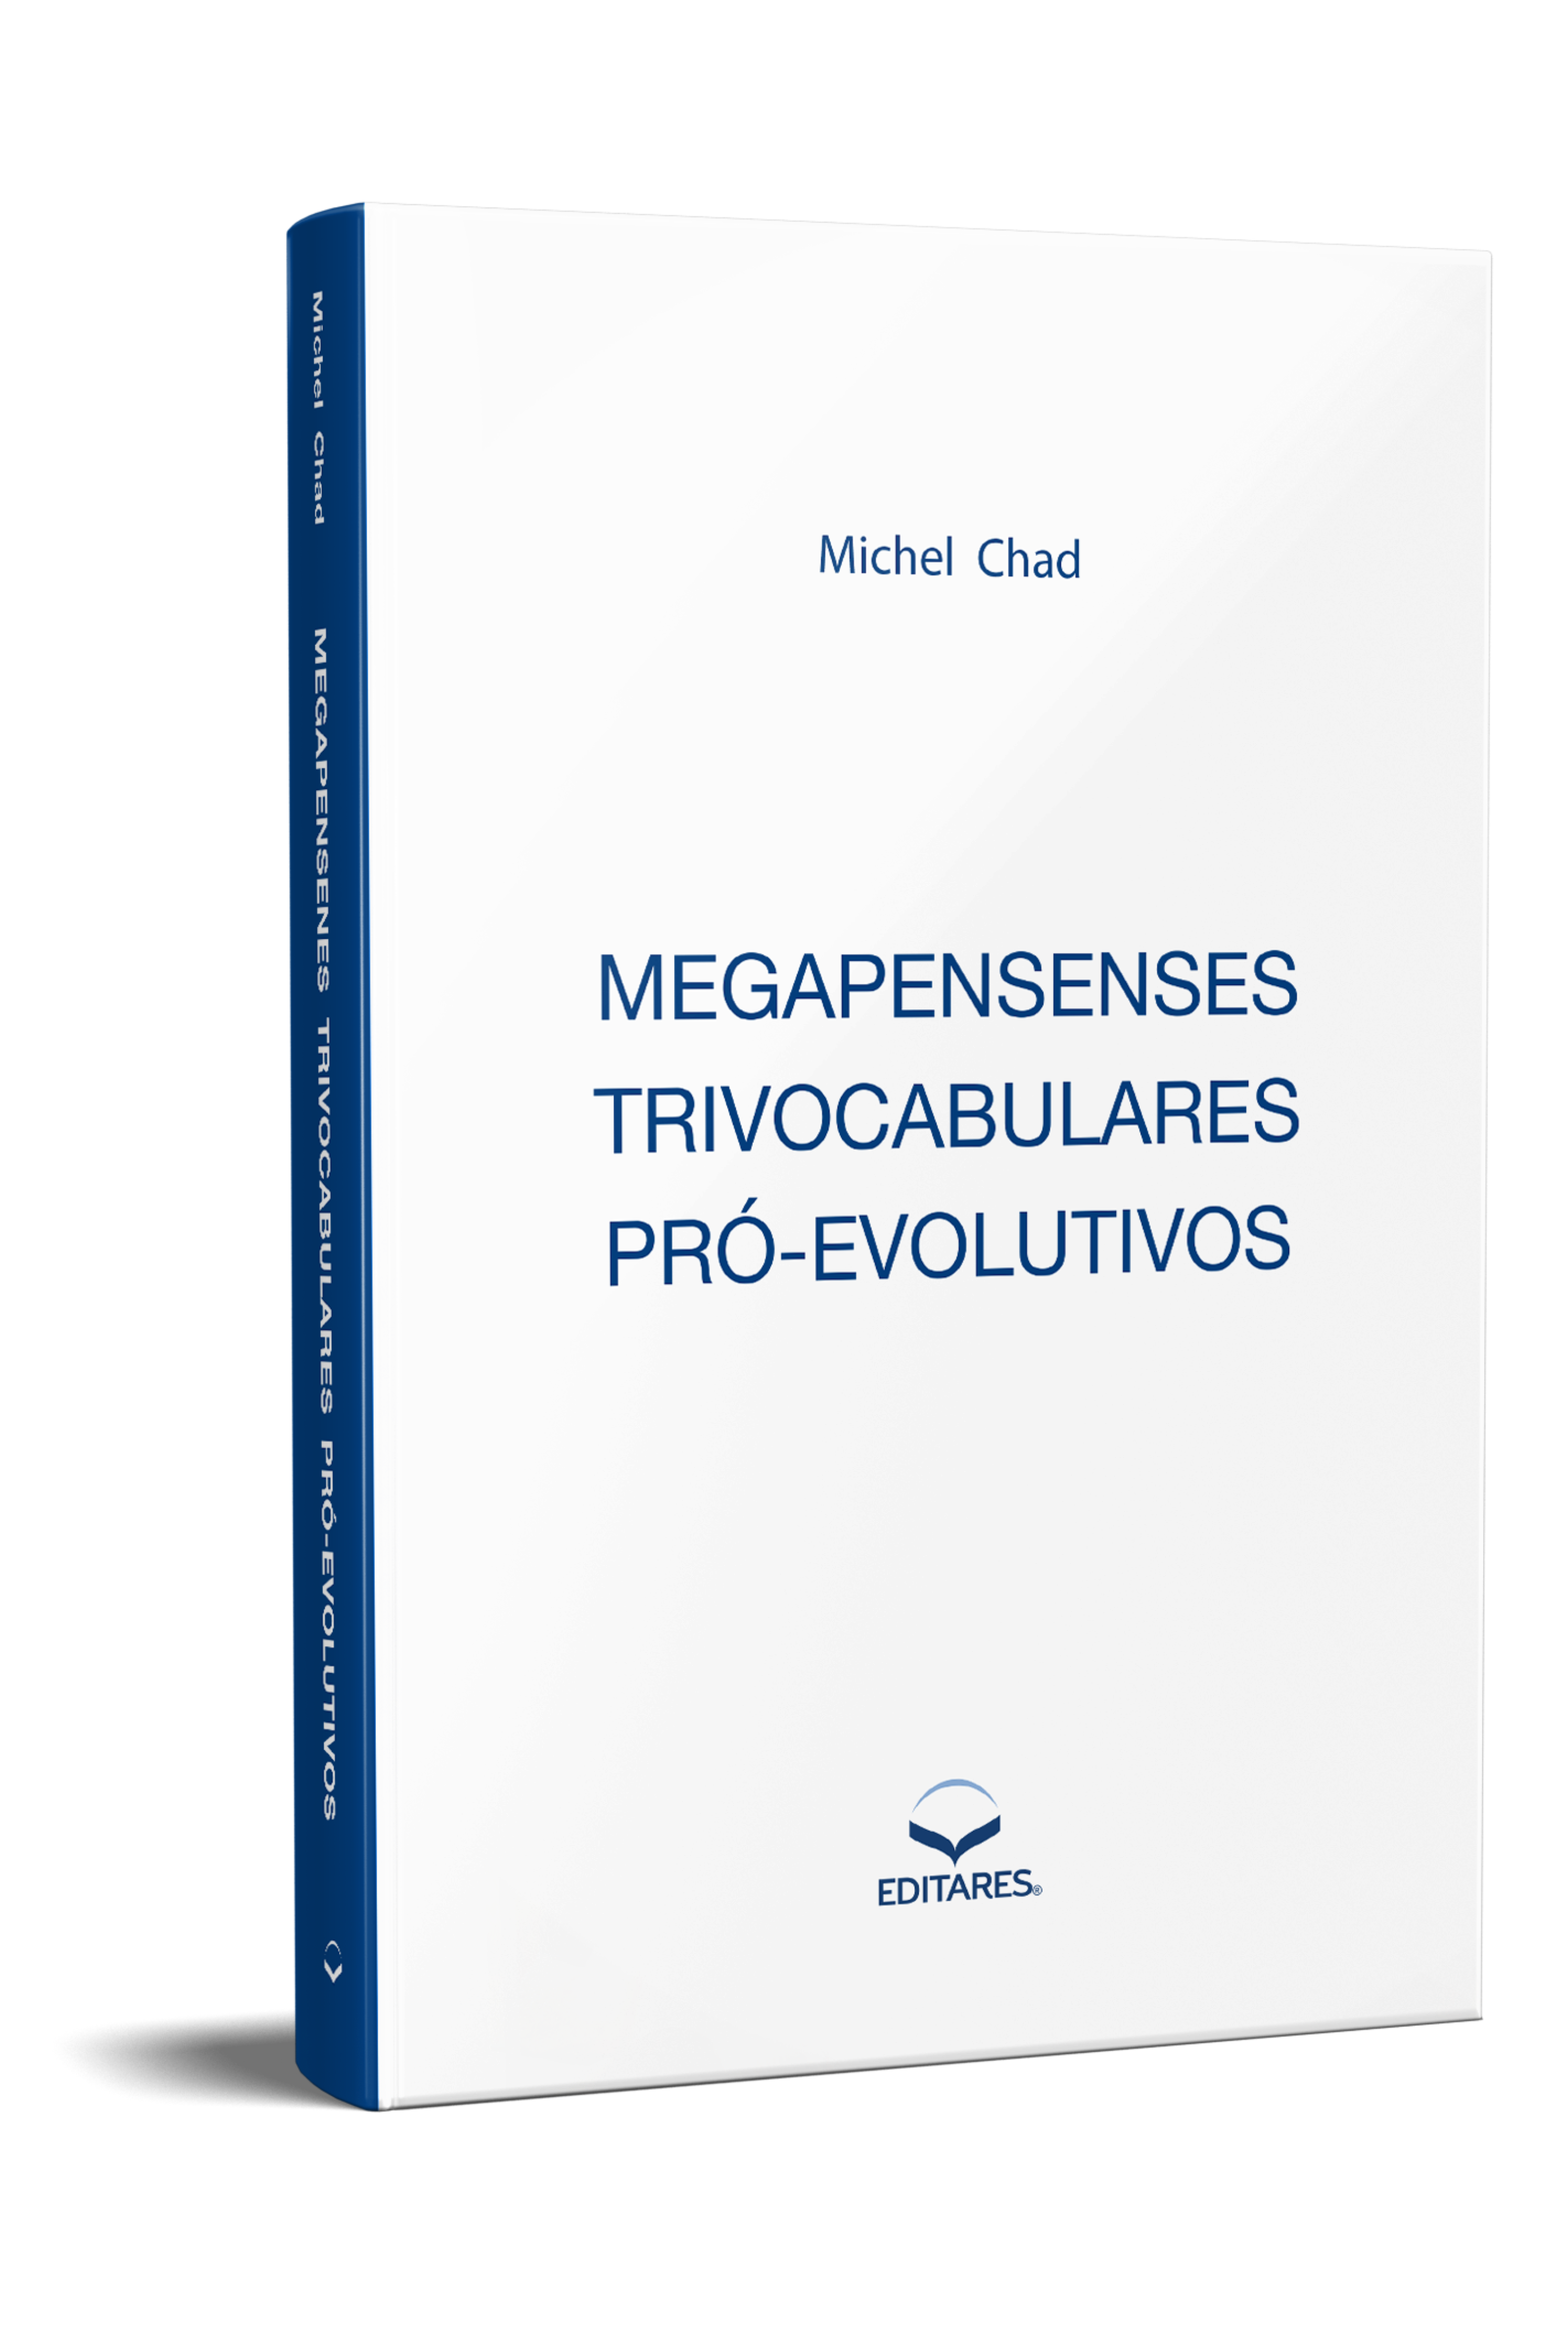
\includegraphics[width=8cm]{articles/entrevista/mockups/Michel-Chad.png}
\end{center}

\textbf{1.       Qual foi a motivação para a escrita da obra? Por que a definição deste tema para publicação de um livro?}

Sou voluntário do IIPC desde 1996. Desde que Waldo Vieira apresentou esta técnica em um curso avançado ministrado em São Paulo, comecei a estudar os megapensenes trivocabulares e elaborar meus próprios. 

Nesta época participava do \textit{Grupo de Pesquisa da Conscienciologia} (GPC) do livro de Waldo Vieira,  \textit{700 Experimentos da Conscienciologia.} Tínhamos encontros semanais de estudo prévio de 2 capítulos do tratado e, na reunião, criávamos uma pensata sobre cada um dos capítulos. Posteriormente, o desafio era formular uma nova frase síntese juntando as duas anteriores. Diversas vezes criamos megapensenes trivocabulares nesta tarefa. 

Talvez pela minha formação em Engenharia Química, o processo de confecção das pensatas trivocabulares e suas 200 fórmulas apresentadas no
\textit{Manual de Megapensenes Trivocabulares,} de Waldo Vieira,  fascinou-me. Pela leitura crítica deste material, busquei aprender e utilizar, na confecção dos meus megapensenes, todas as fórmulas descritas. Inclusive no meu livro proponho 6 fórmulas inéditas criadas por mim.

Outra gescon que serviu como modelo  para minha obra, foi o livro \textit{Megapensenes Trivocabulares da Interassistencialidade,} de Aline Niemeyer, publicado em 2016.

Participei do curso Técnica de Mais 1 ano de Vida Intrafísica, em 2016 e 2017,  ministrado pelo CEAEC, no qual uma das minhas metas foi a escrita e publicação de uma obra com megapensenes trivocabulares. Meta finalmente cumprida em 2024.

\textbf{2.       Quais foram as principais percepções, intra e extrafísicas, durante a pesquisa e a escrita da obra? E posterior ao lançamento?}

Penso que entre as gescons que me propus no meu curso intermissivo, uma delas está relacionada com a produção de neopensatas trivocabulares. 

\begin{pullquote}
    ``Penso que entre as gescons que me propus no meu curso intermissivo, uma delas está relacionada com a produção de neopensatas trivocabulares.''
\end{pullquote}

\textbf{3.       Qual o maior aprendizado com a escrita desta obra?}

Cito entre os benefícios no estudo e elaboração dos megapensenes trivocabulares: ampliação dos diversos dicionários cerebrais, inclusive o analógico; aprimoramento do atributo da associação de ideias; aprofundamento no pensar; comunicação interassistencial sintética; criação do hábito de compor sínteses; desassédio mental; desenvolvimento da criticidade; facilitação da criação e compreensão de neologismos; flexibilidade pensênica; hábito das ponderações das verpons; indução da criatividade.


\textbf{4.       O que poderia dizer como incentivo para que mais pesquisadores invistam na publicação de obras conscienciológicas?}

Finalizo agradecendo a todas as consciências envolvidas neste projeto sugerindo aos interessados estudarem a fundo as 200 fórmulas apresentadas no livro e desenvolverem os seus próprios megapensenes trivocabulares. Elabore neopensatas trivocabulares.


\begin{pullquote}
``Elabore neopensatas trivocabulares.''
\end{pullquote}
    
    \end{multicols}
\end{document}



    \documentclass{gescons}

\genre {Entrevista}
\author{Paula Gabriella Barbosa}
\title{Autoinversão Existencial: Compreensão e~Vivência}
\paginaurl{https://www.youtube.com/live/0akzpk8ifHI}

\begin{document}
    \makeentrevistatitle
    \coverart{back/Paula_Gabriela}

    \begin{multicols}{2}


%\noindent\includegraphics[width=9cm, height=10cm]{example-image} 

\begin{center}
    \includegraphics[width=7cm]{articles/entrevista/mockups/Paula}
\end{center}


\textbf{1. Qual foi a~motivação para a~escrita da obra? Por que a~definição deste tema para publicação de um livro?}

Minha principal motivação foi compartilhar aprendizados obtidos na aplicação prática da técnica da inversão existencial (invéxis), com o~objetivo de auxiliar os leitores na desdramatização dessa proposta evolutiva. O~título \textit{Autoinversão Existencial: Compreensão e~Vivência} reflete a~abordagem intraconsciencial adotada na obra, priorizando os efeitos evolutivos da técnica em detrimento de posturas pro forma. Busquei trazer uma visão mais realista e~experiencial, centrada na autorreflexão e~no autoenfrentamento cosmoético.

\begin{pullquote}
    ``O título Autoinversão Existencial: Compreensão e~Vivência reflete a~abordagem intraconsciencial adotada na obra, priorizando os efeitos evolutivos da técnica em detrimento de posturas pró forma.''
\end{pullquote}

\textbf{2. Quais foram as principais percepções, intra e~extrafísicas, durante a~pesquisa e~a~escrita da obra? E~posterior ao lançamento?}

Durante o~processo de escrita, percebi forte presença e~amparo de consciências extrafísicas com paravisual e~holopensene de matriz oriental, especialmente chinesa. Essa influência se manifestou tanto na leveza da abordagem quanto na clareza reflexiva do conteúdo, favorecendo o~desassédio pessoal e~o~da própria obra. Senti que a~escrita ocorreu em conjunto com os amparadores, dada a~rapidez e~fluidez da redação e~editoração. Considero que houve um investimento extrafísico significativo para que o~livro se materializasse neste momento evolutivo.

\begin{pullquote}
    ``Considero que houve um investimento extrafísico significativo para que o~livro se materializasse neste momento evolutivo.''
\end{pullquote}

\textbf{3. Qual o~maior aprendizado com a~escrita desta obra?}

O principal aprendizado foi compreender o~valor da escrita como forma de posicionamento multidimensional. Através deste livro, consegui expressar de maneira clara meu entendimento sobre a~técnica da invéxis, além de assumir um posicionamento mais lúcido diante do meu retrogrupo de base religiosa. Também entendi que, independentemente de onde eu esteja, a~obra continuará disponível para as consciências interessadas, mantendo vivas as ideias e~experiências compartilhadas.

\textbf{4. O~que poderia dizer como incentivo para que mais pesquisadores invistam na publicação de obras conscienciológicas?}

A escrita conscienciológica é~uma oportunidade de renovação da autoimagem, além de constituir um posicionamento multidimensional diante do tema abordado. Ao escrever, o~pesquisador amplia o~alcance assistencial de suas vivências e~reciclagens. Publicar é~uma forma de fixar marcos na própria trajetória e,~ao mesmo tempo, abrir caminhos para outras consciências.
    
    
    \end{multicols}
\end{document}





    \documentclass{gescons}

\genre {Entrevista}
\author{Ricardo Rezende}
\title{Autoidentificação Proexológica}

\begin{document}
    \makeentrevistatitle

    \begin{multicols}{2}


%\noindent\includegraphics[width=9cm, height=10cm]{example-image} 
\begin{center}
    \includegraphics[width=8cm]{articles/entrevista/mockups/Ricardo-Rezende-Proexis.png}
\end{center}

\textbf{1. Qual foi a motivação para a escrita da obra? Por que a definição deste tema para publicação de um livro? }

A ideia de escrever esta obra surgiu em diálogo extrafísico com consciex amparadora, autorrememorada após o despertamento físico. A paraindicação dessa autogescon causou surpresa desconfortável porque não pensava em escrever livro nessa temática e estava priorizando outro trabalho gesconográfico. Apesar disso, desde jovem, confio, coopero com os amparadores extrafísicos e não pretendo mudar esse ortoposicionamento. Assim, acatei a paratarefa.

\begin{pullquote}
    ``A paraindicação dessa autogescon causou surpresa desconfortável porque não pensava em escrever livro nessa temática e estava priorizando outro trabalho gesconográfico''
\end{pullquote}

\textbf{2. Quais foram as principais percepções, intra e extrafísicas, durante a pesquisa e a escrita da obra? }

No decorrer da redação dos capítulos da obra, para a criação dos conteúdos era necessária rever situações marcantes do próprio passado, ao modo de retrospectivação autobiográfica, relativas as memórias intermissivas e retrovidas pessoais. Nesse processo de revisão e análise de retrofatos particulares, constatava estar juntando, ordenando e encaixando no lugar certo as peças de complexo quebra-cabeças autoconscienciológico, sob os ângulos da \textit{Proexologia, Duplologia, Extrafisicologia, Intermissiologia e Holobiografologia}.

\textbf{3. Qual o maior aprendizado com a escrita desta obra? }

A compreensão aprofundada sobre a identificação e o desenvolvimento da autoproéxis.

\textbf{4. O que poderiam dizer como incentivo para que mais pesquisadores invistam na publicação de obras conscienciológicas?}

O hábito da escrita conscienciológica com publicações seriadas resulta na ampliação dinâmica da hiperacuidade e na sustentação da conexão profícua com os amparadores extrafísicos e o holopensene homeostático da autoparaprocedência cursista, favorecendo o desenvolvimento intraconsciencial e da interassistencialidade tarística.

\begin{pullquote}
    ``O hábito da escrita conscienciológica com publicações seriadas resulta na ampliação dinâmica da hiperacuidade e na sustentação da conexão profícua com os amparadores extrafísicos e o holopensene homeostático da autoparaprocedência cursista.''
\end{pullquote}
    
    \end{multicols}
\end{document}



    \documentclass{gescons}

\genre {Entrevista}
\author{Ricardo Rezende}
\title{Ortoprincípios Norteadores da Invéxis}

\begin{document}
    \makeentrevistatitle
    \coverart{back/Ricardo_Rezende_Ortoprincipios}

\begin{center}
    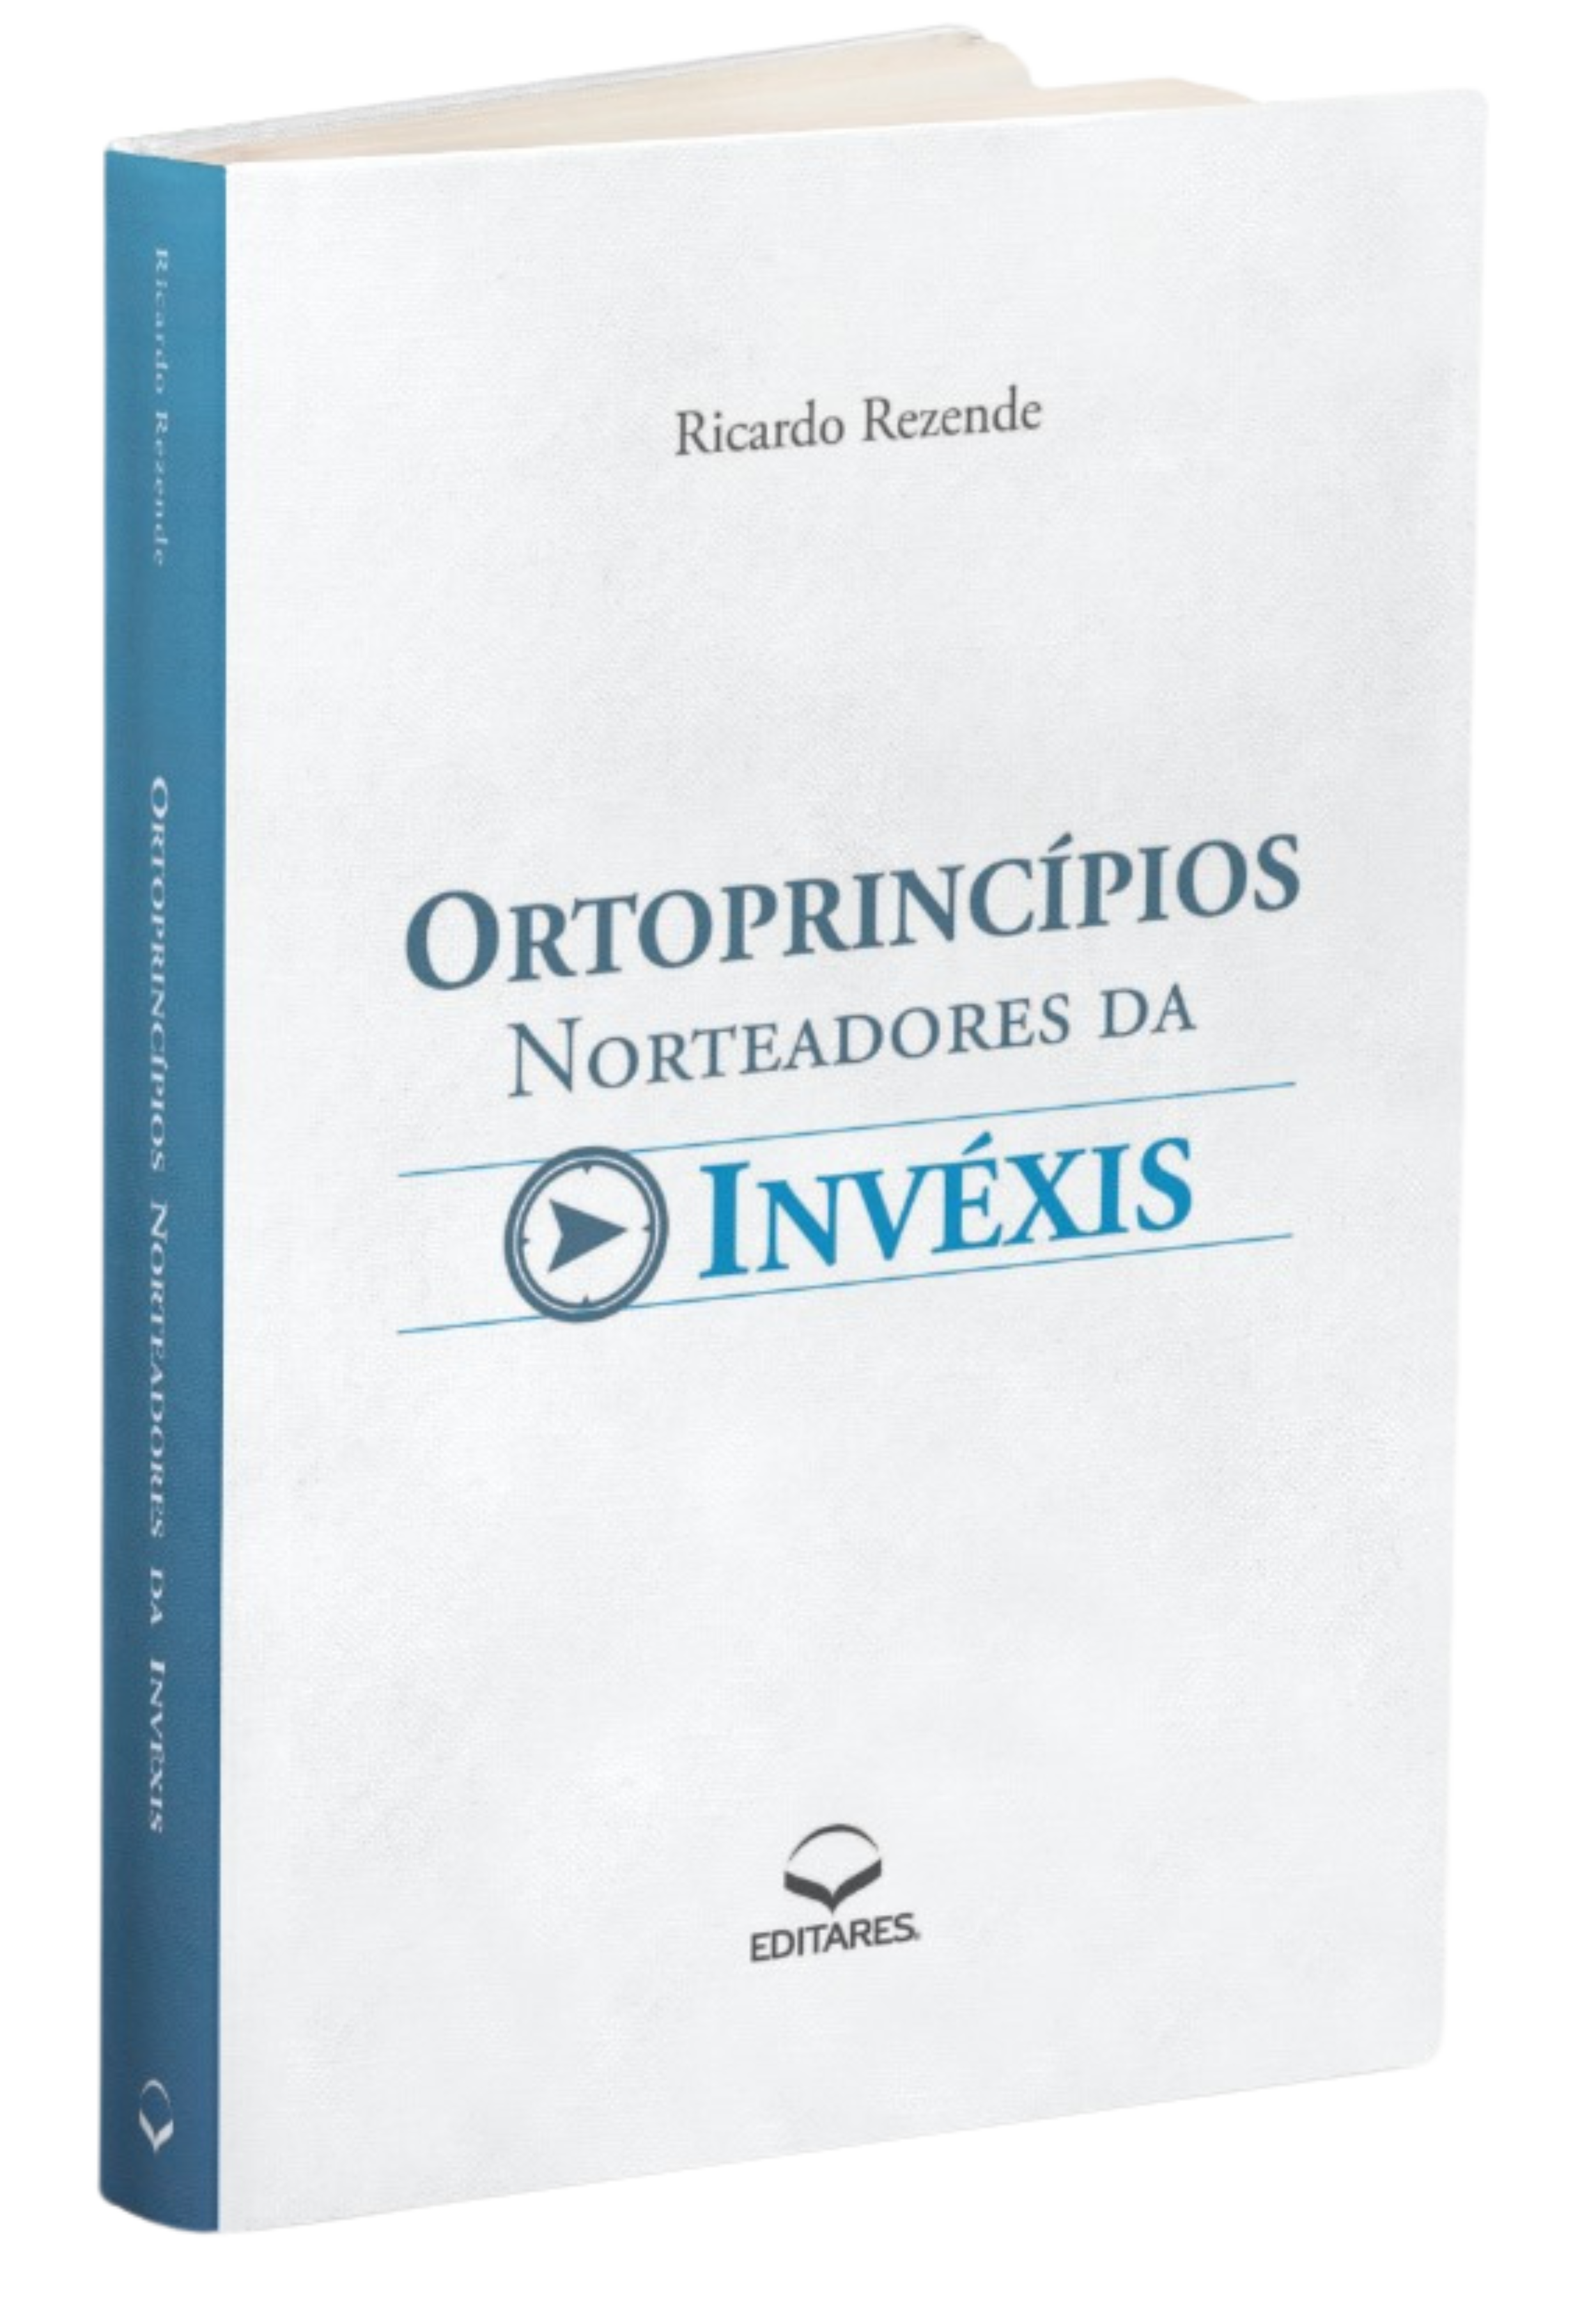
\includegraphics[width=7cm]{articles/entrevista/mockups/Ricardo-Rezende-Invexis.png}
\end{center}

    \begin{multicols}{2}


%\noindent\includegraphics[width=9cm, height=9cm]{example-image} 

\textbf{1. Qual foi a motivação para a escrita da obra? Por que a definição deste tema para publicação de um livro?}

Desde junho de 2022, este autor iniciou a escrita de verbetes a respeito de temas de Invexologia, incentivado pelo início dos trabalhos voluntários pessoais na Assinvéxis. Nesse período, houve imersão ou saturação intelectiva homeostática quanto aos conteúdos sobre inversão existencial, por meio da dedicação à verbetografia, resultando no estudo do tema \textit{holofilosofia da invéxis}.

Mais adiante para compreender melhor o assunto, iniciou-se mapeamento para identificar quais princípios cosmoéticos ou as \textit{condições evoluídas de se viver} poderiam compor a filosofia teática da inversão existencial. Para isso, realizou-se pesquisas em publicações conscienciológicas buscando localizar nos fundamentos ou nas bases teórico-práticas da Invexologia os ortoprincípios constituintes, de modo a estruturar a tese central da obra \textit{Ortoprincípios Norteadores da Invéxis}.

Portanto, essa obra advém da curiosidade pesquisística e determinação grafopensênica com o propósito de descortinar a filosofia teática da invéxis, sob 
o ângulo interdisciplinar de 5 especialidades: Principiologia, Experienciologia, Traforologia, Evoluciologia e Seriexologia.

\begin{pullquote}
``Essa obra advém da curiosidade pesquisística e determinação grafopensênica com o propósito de descortinar a filosofia teática da invéxis.''    
\end{pullquote}




\textbf{2. Qual o maior aprendizado com a escrita desta obra?}

A compreensão aprofundada da holofilosofia da invéxis, a expansão da paracognição invexológica e da lucidez invexometrológica pessoal.

\textbf{3. O que poderiam dizer como incentivo para que mais pesquisadores invistam na publicação de obras conscienciológicas?}

O hábito da escrita conscienciológica com publicações seriadas resulta na ampliação dinâmica da hiperacuidade e na sustentação da conexão profícua com os amparadores extrafísicos e o holopensene homeostático da autoparaprocedência cursista, favorecendo o desenvolvimento intraconsciencial e da interassistencialidade tarística.


    
    
    \end{multicols}


\end{document}


    \documentclass{gescons}

\genre {Entrevista}
\author{Roberta Bouchardet}
\title{Interassistência: Teoria e~Prática Sob a~Ótica da Conscienciologia}
\paginaurl{https://www.youtube.com/live/zasm7A2swDQ}

\begin{document}
    \makeentrevistatitle
    \coverart{back/Roberta_Bouchardet}

    \begin{multicols}{2}

\begin{center}
    \includegraphics[width=7cm]{articles/entrevista/mockups/Roberta-Bouchardet}
\end{center}

%\begin{center}
%    \includegraphics[width=8cm]{articles/entrevista/mockups/Roberta-Bouchardet}
%\end{center}

\textbf{1.       Qual foi a~motivação para a~escrita da obra? Por que a~definição deste tema para publicação de um livro?}

Sempre gostei de livros e~de escrever. E~assim, junto com o~incentivo do Prof. Waldo em deixar uma gestação consciencial nessa existência, veio a~motivação de registrar parte do conhecimento adquirido em tantas décadas de estudo e~autopesquisas na Conscienciologia. A~definição do tema veio aos poucos. Começou com o~verbete Autoamparo, que deveria ser a~base do livro, mas a~temática cresceu e~se tornou Interassistência, sendo o~Autoamparo um dos capítulos do livro.

\textbf{2.       Quais foram as principais percepções, intra e~extrafísicas, durante a~pesquisa e~a~escrita da obra? E~posterior ao lançamento?}

Já há alguns anos eu estava escrevendo alguns capítulos, sem saber ainda o~escopo da obra, e~no Acoplamentarium de pesquisa, durante uma prática energética, tive o~fenômeno de captação de ideias e~visualizei todo o~sumário, os capítulos a~serem escritos. Anotei tudo e~a~partir daí a~escrita fluiu bem mais rapidamente. Durante a~escrita, sentia-me muito motivada e~energizada, o~mentalsoma não cansava. O~que cansava era o~soma, que exigia parar. Após o~lançamento, percebo mudanças pensênicas, maior tranquilidade, talvez novos amparadores, o~que está em avaliação ainda.

\begin{pullquote}
    ``Durante a~escrita, me sentia muito motivada e~energizada, o~mentalsoma não cansava''
\end{pullquote}


\textbf{3.       Qual o~maior aprendizado com a~escrita desta obra?}

Aprendi muito sobre o~processo de organização de uma obra para publicação. Uma coisa é~escrever textos para nós mesmos ou trabalhos para cursos. Outra, muito diferente, é~o~livro. Muitas etapas são necessárias e~muitas pessoas são envolvidas e~trabalham arduamente junto com o~autor. Durante o~processo, tornei-me participante do Conselho Editorial da Editares e~busco auxiliar outros autores nesse processo. É~preciso persistência e~paciência; a~pressa em fazer rápido acaba assediando o~fluxo e~atrasando mais ainda os trabalhos. É~preciso trabalhar ombro a~ombro, tanto com os amparadores extrafísicos, como também com os colegas intrafísicos nas várias etapas de edição do livro. Entrar em conflito é~contraproducente.

\begin{pullquote}
    ``É preciso persistência e~paciência; a~pressa em fazer rápido acaba assediando o~fluxo e~atrasando mais ainda os trabalhos.''
\end{pullquote}

\textbf{4.       O~que poderia dizer como incentivo para que mais pesquisadores invistam na publicação de obras conscienciológicas?}

Escolha uma temática de interesse, busque bibliografia em todas as bases de consulta da Conscienciologia e~comece a~focar naquele assunto. Busque convergir as atividades para aquela temática, anote as experiências. Antes de começar a~escrever, defina o~escopo, a~estrutura do livro e~o~público-alvo. E~busque assessoria da Uniescon. Há várias atividades na IC para ajudar o~autorando. 
    
    
    \end{multicols}
\end{document}



    \documentclass{gescons}

\genre {Editorial}
\title {Hello world}
\author{Abdullah José Kim}

\begin{document}
    \maketitle

    \fullwidthimage{fields}{b}

    \begin{multicols}{3}
        \begin{lead}
            \lipsum[1]
        \end{lead}

        \lipsum[2-3]
        
        \begin{pullquote}
            ``If you cannot do great things, do small things in a~great way.'' amanda
        \end{pullquote}
        
        \lipsum[4]
        
    \end{multicols}
\end{document}

    \documentclass{gescons}

\genre {Science}
\title {Engineer becomes famous after building first-ever PUNDITECTOR}
\author{Fanny Furling}

\begin{document}
    \maketitle
    
    \begin{lead}
        \lipsum[1]
    \end{lead}
    
    \begin{multicols}{3}
        \lipsum[2-11]
    \end{multicols}
    
    \begin{figure}
        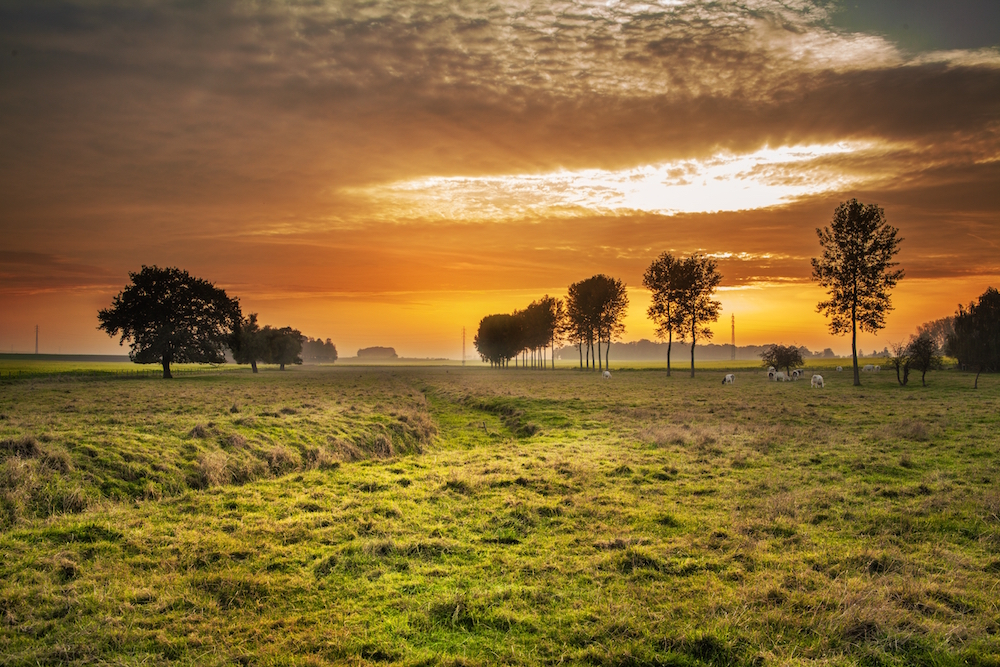
\includegraphics[width=\textwidth]{landscape}
    \end{figure}
\end{document}

    \documentclass{gescons}

\genre {Economy}
\title {Retired fundamentalists infuriated by government's decision to declare total workfare}
\author{Kane Keynes}

\begin{document}
    \maketitle

    
    
    
    \begin{multicols}{2}
        \begin{lead}
            \lipsum[1]
        \end{lead}

        \lipsum[2]
        
        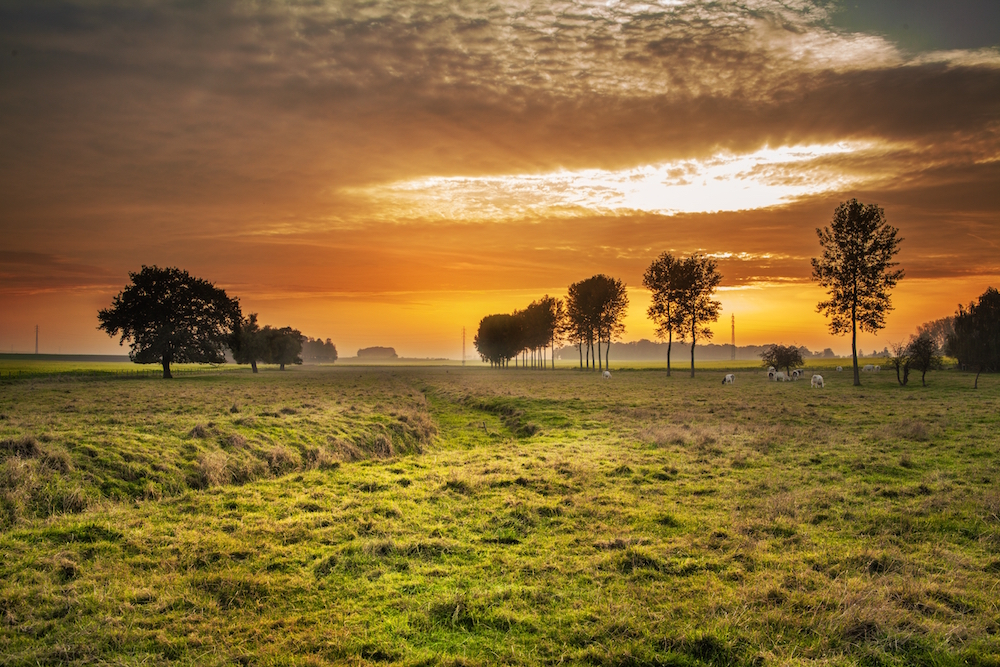
\includegraphics[width=\columnwidth]{landscape}
        
        \lipsum[3-6]
    \end{multicols}
\end{document}

    \documentclass{gescons}

\genre {Feature story}
\title {Is broccoli from outer space?}
\author{Dwight Greenman}

\begin{document}
    \makecovertitle{broccoli}{\lipsum[1]}

    \begin{multicols}{3}

        \lipsum[2-8]
        
        \lipsum[9-18]
        
        No.
    \end{multicols}
\end{document}


    \fullpageadvertisement{images/amigos-da-enciclopedia}{10}{10}
\end{document}
